\documentclass[a4paper,10pt]{article}
\usepackage[utf8]{inputenc}
\usepackage{polski}
\usepackage{graphicx}
\usepackage{listings}
\usepackage[usenames,dvipsnames]{color}
\addtolength{\hoffset}{-1cm}
\addtolength{\voffset}{-2cm}
\addtolength{\textwidth}{2cm}
\addtolength{\textheight}{3cm}
\usepackage{setspace}
\usepackage{indentfirst}
\usepackage{graphicx}
\lstset{
    language=Matlab,
    basicstyle=\scriptsize,
    aboveskip={1.5\baselineskip},
    columns=fixed,
    showstringspaces=false,
    extendedchars=true,
    breaklines=true,
    tabsize=4,
    prebreak = \raisebox{0ex}[0ex][0ex]{\ensuremath{\hookleftarrow}},
    frame=single,
    showtabs=false,
    showspaces=false,
    showstringspaces=false,
    identifierstyle=\ttfamily,
    keywordstyle=\color[rgb]{0,0,1},
    commentstyle=\color[rgb]{0.133,0.545,0.133},
    stringstyle=\color[rgb]{0.627,0.126,0.941},
    numbers=left,
    numberstyle=\tiny,
    stepnumber=1,
    numbersep=5pt,
    captionpos=b,
    escapeinside={\%*}{*)}
}

\def\figurename{Rys.}
\def\lstlistingname{Fun.}

\title{Informatyczne Systemy Sterowania \\ \large Ćwiczenie 2: Systemy regulacji - Regulator PID}

\author{Adam Jordanek 168139, Tomasz Klimek 168092}

\begin{document}
\maketitle

\section{Wstęp}\label{sec:wstęp}
\subsection{Cel ćwiczenia}
Celem tego ćwiczenia jest poznanie podstawowej struktury systemu sterowania z typową formą algorytmu regulacji PID, oraz zapoznanie się z częścią pakietu M\small ATLAB \normalsize - Simulinkiem, oraz jego możliwości w zakresie modelowania i analizy systemów regulacji.
%Więcej?

\subsection{Plan badań} 
\begin{enumerate}
	\item Symulacja systemu regulacji
	\begin{enumerate}
		\item Regulator P. Zbadać wpływ wartości wzmocnienia regulatora na działanie systemu. 
	    \item Regulator   PI.   Zbadać  wpływ   wartości   parametru   całkowania   na   działanie   systemu 
       (dla ustalonej wartości parametru $k$). 
    	\item Regulator PID. Zbadać wpływ wartości parametru różniczkowania na działanie 
       systemu (dla ustalonych wartości parametrów $k$ i $T_i$). 
	\end{enumerate}
	\item Dobór optymalnych parametrów regulatora. Sporządzenie wykresów:
	\begin{enumerate}
		\item dla regulatora P. 
    	\item dla regulatora PI przy trzech różnych ustalonych wartościach parametru $k$.  
    	\item dla regulatora PID przy trzech różnych wartościach parametru oraz ustalonej wartości parametru $k$.
	\end{enumerate}
	\item Dobór parametrów regulatora PID według zasad Zieglera–Nicholsa
	\begin{enumerate}
		\item Doświadczalnie znaleźć współczynnik wzmocnienia, dla którego układ traci stabilność.
		\item Ustalić okres oscylacji i wzmocnienie krytyczne.
		\item Według odpowiednich rekomendacji określić wartości parametrów regulatora PID.
	\end{enumerate}
\end{enumerate}
Zadania należy wykonać dla obiektu o podanej transmitancji operatorowej:
\begin{equation} \label{eqn:transOS}
	G(s) = \frac{b}{s^3 + a_2 s^2 + a_1 s + a_0}
\end{equation}
%Copy/Paste z treści zadania...

\newpage
\section{Realizacja planu i wyniki}

%---------------------------------------------------------------------------------------------------------------------
%
%ZADANIE 1
%
%---------------------------------------------------------------------------------------------------------------------
\subsection{Symulacja systemu regulacji.}\label{sec:zad1}
System regulacji będziemy symulować przy użyciu programu Simulink będącego częścią pakietu M\small ATLAB. \\
\normalsize Schemat systemu służącego nam do symulacji przedstawiony został na poniższym rysunku.

\begin{figure}[h]
    \centering
	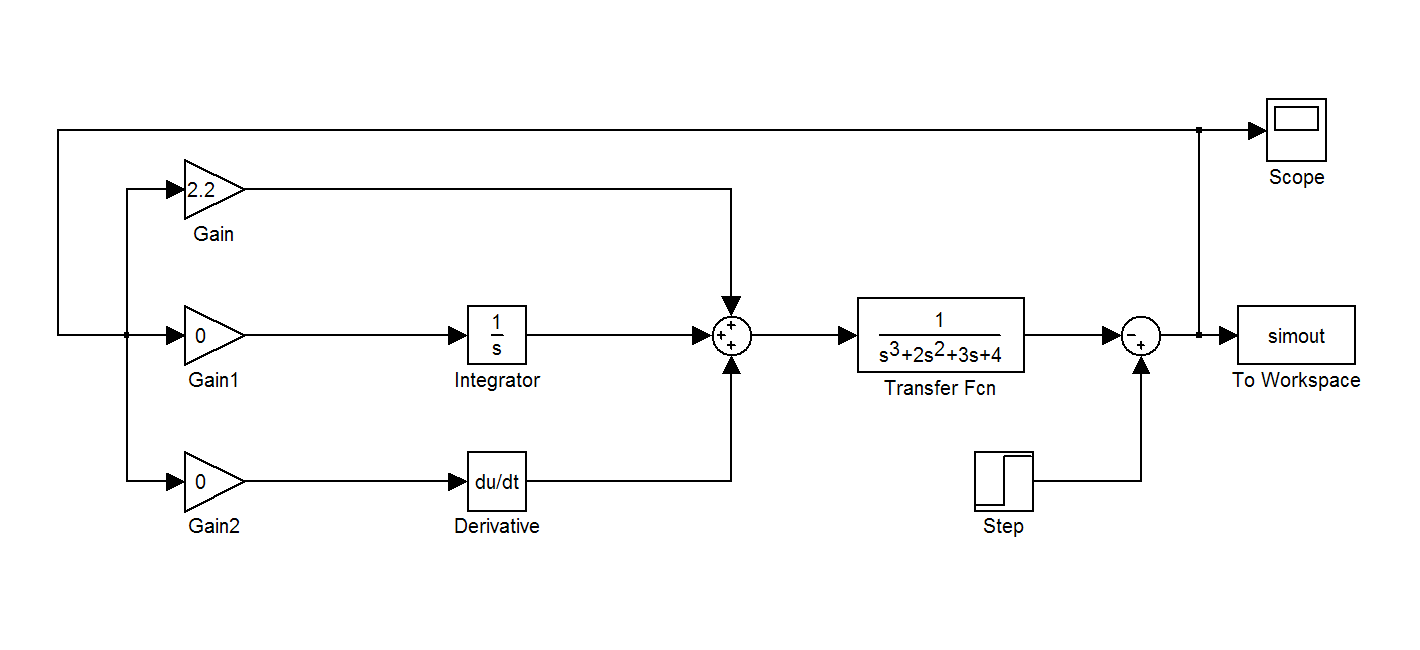
\includegraphics[width=120mm]{CW2-schemat.png}
	\caption{Schemat symulacji obiektu z regulatorem PID}
    \label{fig:Rysunek}
\end{figure}

Wartości błędu regulacji $\varepsilon(t)$ mogą być odczytywane zarówno na wykresie $Scope$ jak i z poziomu M\small ATLABA \normalsize dzięki obiektowi $simout$.

Regulator PID jest opisany następującą transmitancją:
\begin{equation} \label{eqn:transPID}
	G(s) = k + {T_{i} \over s} + T_{d}s ,
\end{equation}
gdzie $k$ to współczynnik wzmocnienia, $T_{i}$ to parametr członu całkującego, a $T_{d}$ to parametr członu różniczkującego.

Podczas ćwiczenia przyjęliśmy następujące wartości parametrów transmitancji obiektu sterowania (\ref{eqn:transOS}): 
\begin{equation} \label{eqn:paramTransOS}
	b = 1,
	a_{2} = 2, 
	a_{1} = 3, 
	a_{0} = 4
\end{equation}
oraz zadanej wartości wyjścia $y^{*} = 1$.

\subsubsection{Regulator P.}\label{sec:regP}
Aby zasymulować regulator P musieliśmy ustawić wartości parametru całkującego i różniczkującego na $T_{i}=0$, $T_{d}=0$. \\
Następnie wykorzystując poniższą funkcję przetestowaliśmy zachowanie regulatora P dla różnych wartości parametru $k$. \\
\begin{lstlisting}[caption=Funkcja testująca regulator P.]
function testP(start, step, stop)
load_system('model.mdl');
hold on;
k = start;
color = char('r', 'k', 'b', 'g', 'y', 'm');
set_param('model/Gain1', 'Gain', num2str(0));
set_param('model/Gain2', 'Gain', num2str(0));
while (k <= stop)
    set_param('model/Gain', 'Gain', num2str(k));
    sim('model.mdl');
    wy = simout.signals.values;
    figure(1);
    plot(tout, wy, 'Color', color(mod(i,6)+1));
    k = k + step;
end
end
\end{lstlisting}
W ten sposób otrzymalismy następujące wykresy: \\
\begin{figure}[!h]
    \centering
	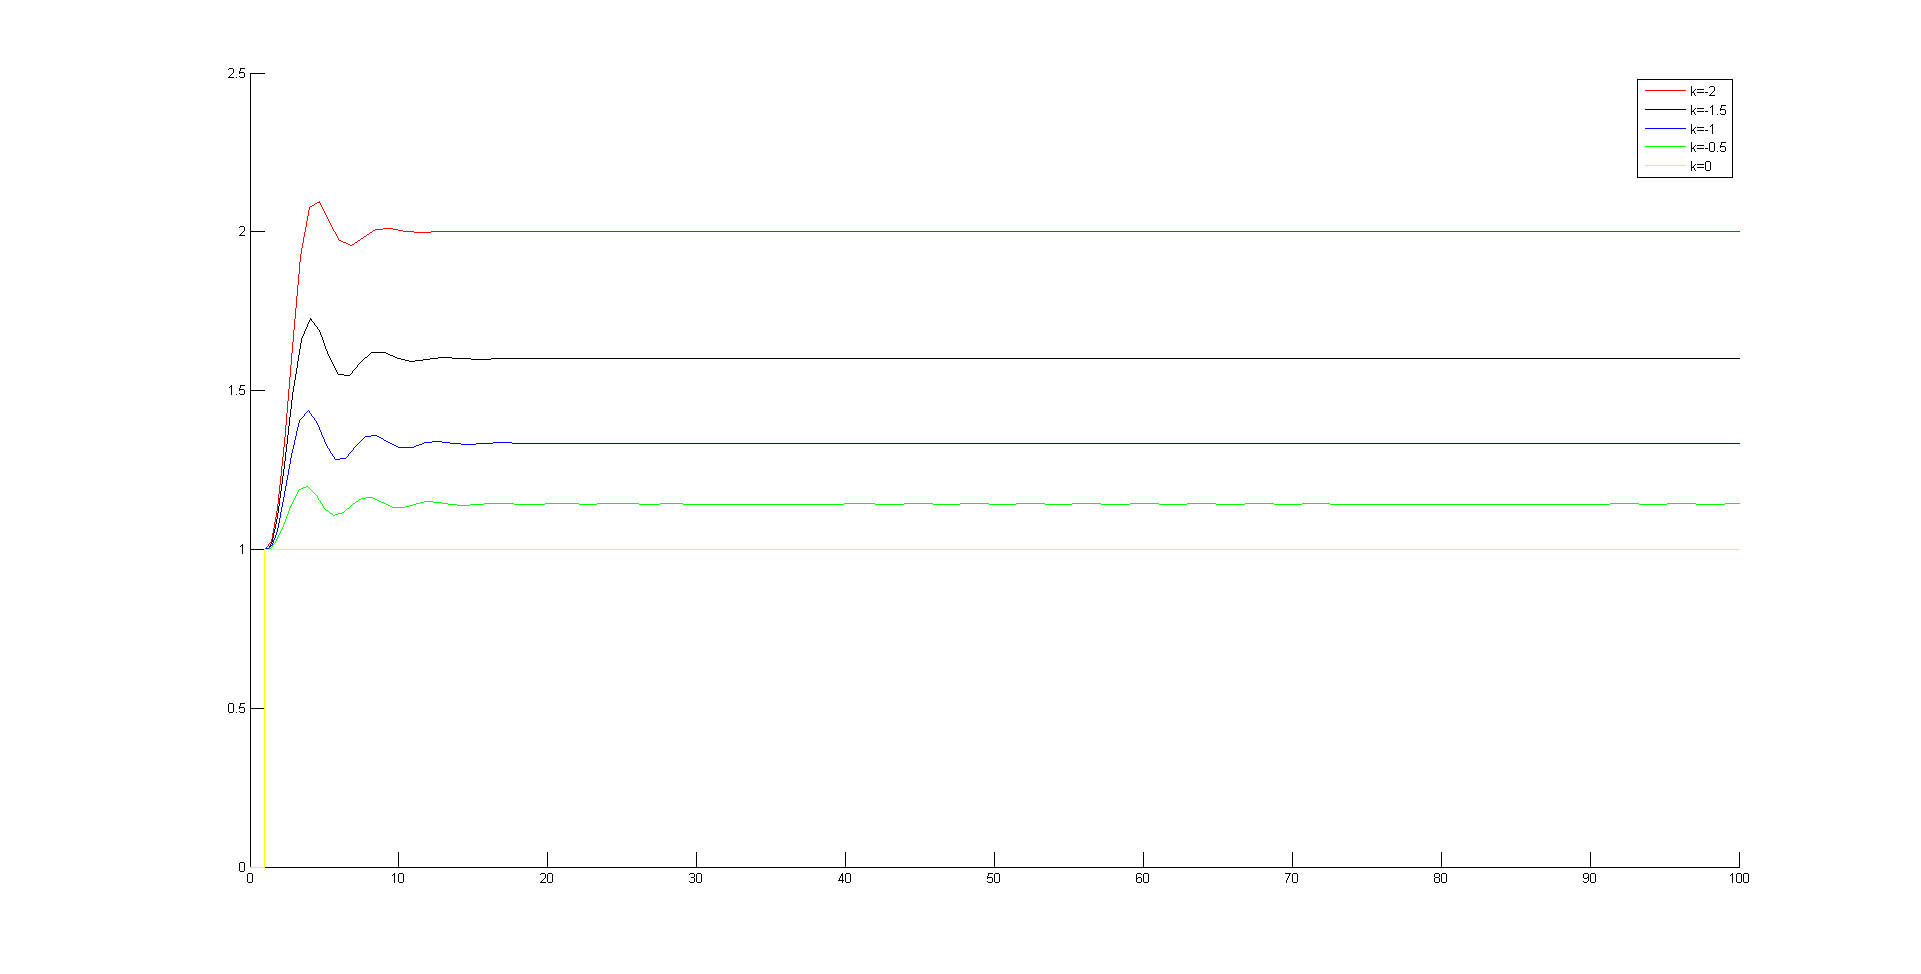
\includegraphics[width=130mm]{CW2-regulatorP-eu.png}
	\caption{Wykres przebiegu funkcji $\varepsilon(t)$ regulatora P dla wartości ujemnych k.}
    \label{fig:regulatorPeu}
\end{figure}
\begin{figure}[!h]
    \centering
	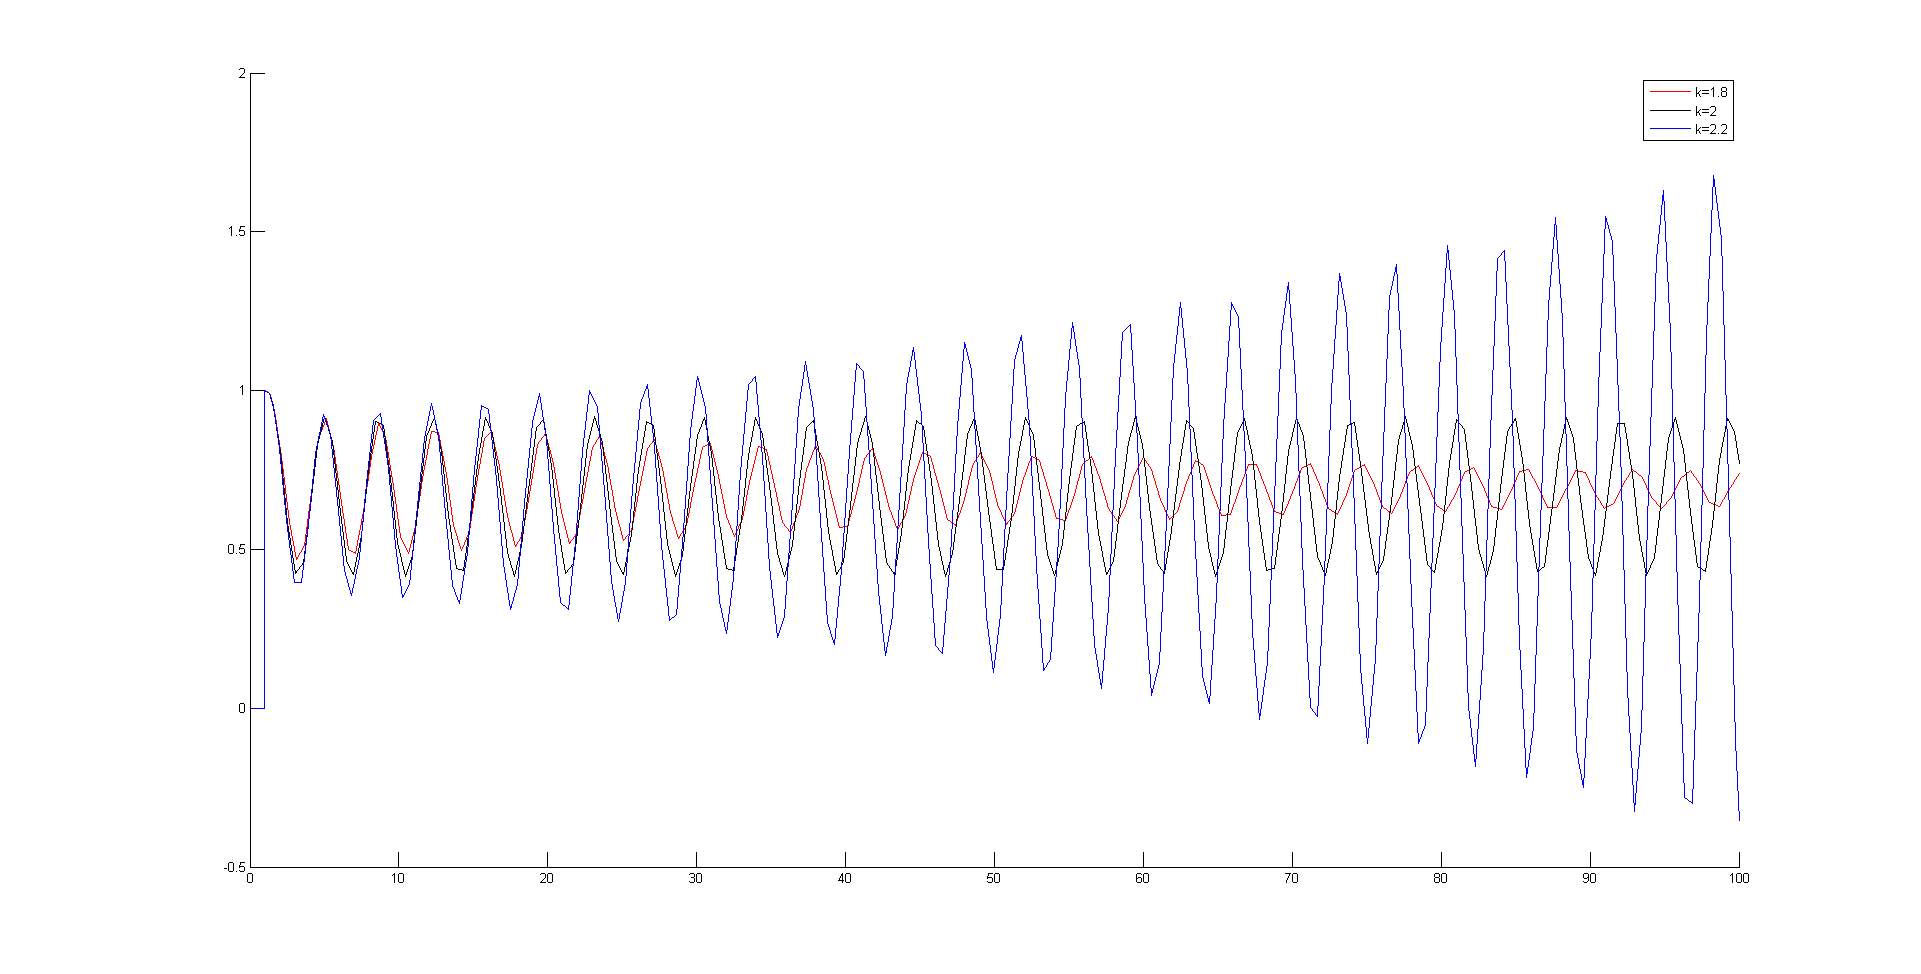
\includegraphics[width=130mm]{CW2-regulatorP-ed.png}
	\caption{Wykres przebiegu funkcji $\varepsilon(t)$ regulatora P dla wartości dodatnich k.}
    \label{fig:regulatorPed}
\end{figure}
\\ Z wykresu \ref{fig:regulatorPeu}, oraz \ref{fig:regulatorPed} możemy zauważyć, że:
\begin{itemize}
	\item Dla ujemnych wartości parametru $k$ drgania po pewnym czasie ustają, a wykres $\varepsilon(t)$ stabilizuje się na pewnym poziomie większym od żądanej wartości $y*$, a poziom ten jest tym większy im mniejsza jest wartość parametru $k$.
	\item Dla wartości dodatnich wykres $\varepsilon(t)$ przyjmuje postać drgań oscylujących wokół wartości ~0.6. Dla wartości $k$ mniejszych od 2 amplituda tych drgań maleje, natomiast rośnie dla wartości większych od 2. Dla $k=2$ amplituda tych drgań jest stała.
	\item Regulator P nie jest efektywny, ponieważ wykres funkcji $\varepsilon(t)$ oscyluje poniżej wartości $y*$, ale nie wokół 0.
\end{itemize}
\subsubsection{Regulator PI.}\label{sec:regPI}
Aby zasymulować regulator PI musieliśmy ustawić wartości parametru proporcjonalnego i różniczkującego na $k=2$, $T_{d}=0$. \\
Następnie wykorzystując poniższą funkcję przetestowaliśmy zachowanie regulatora PI dla różnych wartości parametru $T_{i}=0$. \\
\begin{lstlisting}[caption=Funkcja testująca regulator PI.]
function testPI(start, step, stop)
load_system('model.mdl');
hold on;
ti = start;
color = char('r', 'k', 'b', 'g', 'y', 'm');
set_param('model/Gain', 'Gain', num2str(2));
set_param('model/Gain2', 'Gain', num2str(0));
while (ti <= stop)
    set_param('model/Gain1', 'Gain', num2str(ti));
    sim('model.mdl');
    wy = simout.signals.values;
    figure(1);
    plot(tout, wy, 'Color', color(mod(i,6)+1));
    ti = ti + step;
end
end
\end{lstlisting}
W ten sposób otrzymalismy następujące wykresy: \\
\begin{figure}[!h]
    \centering
	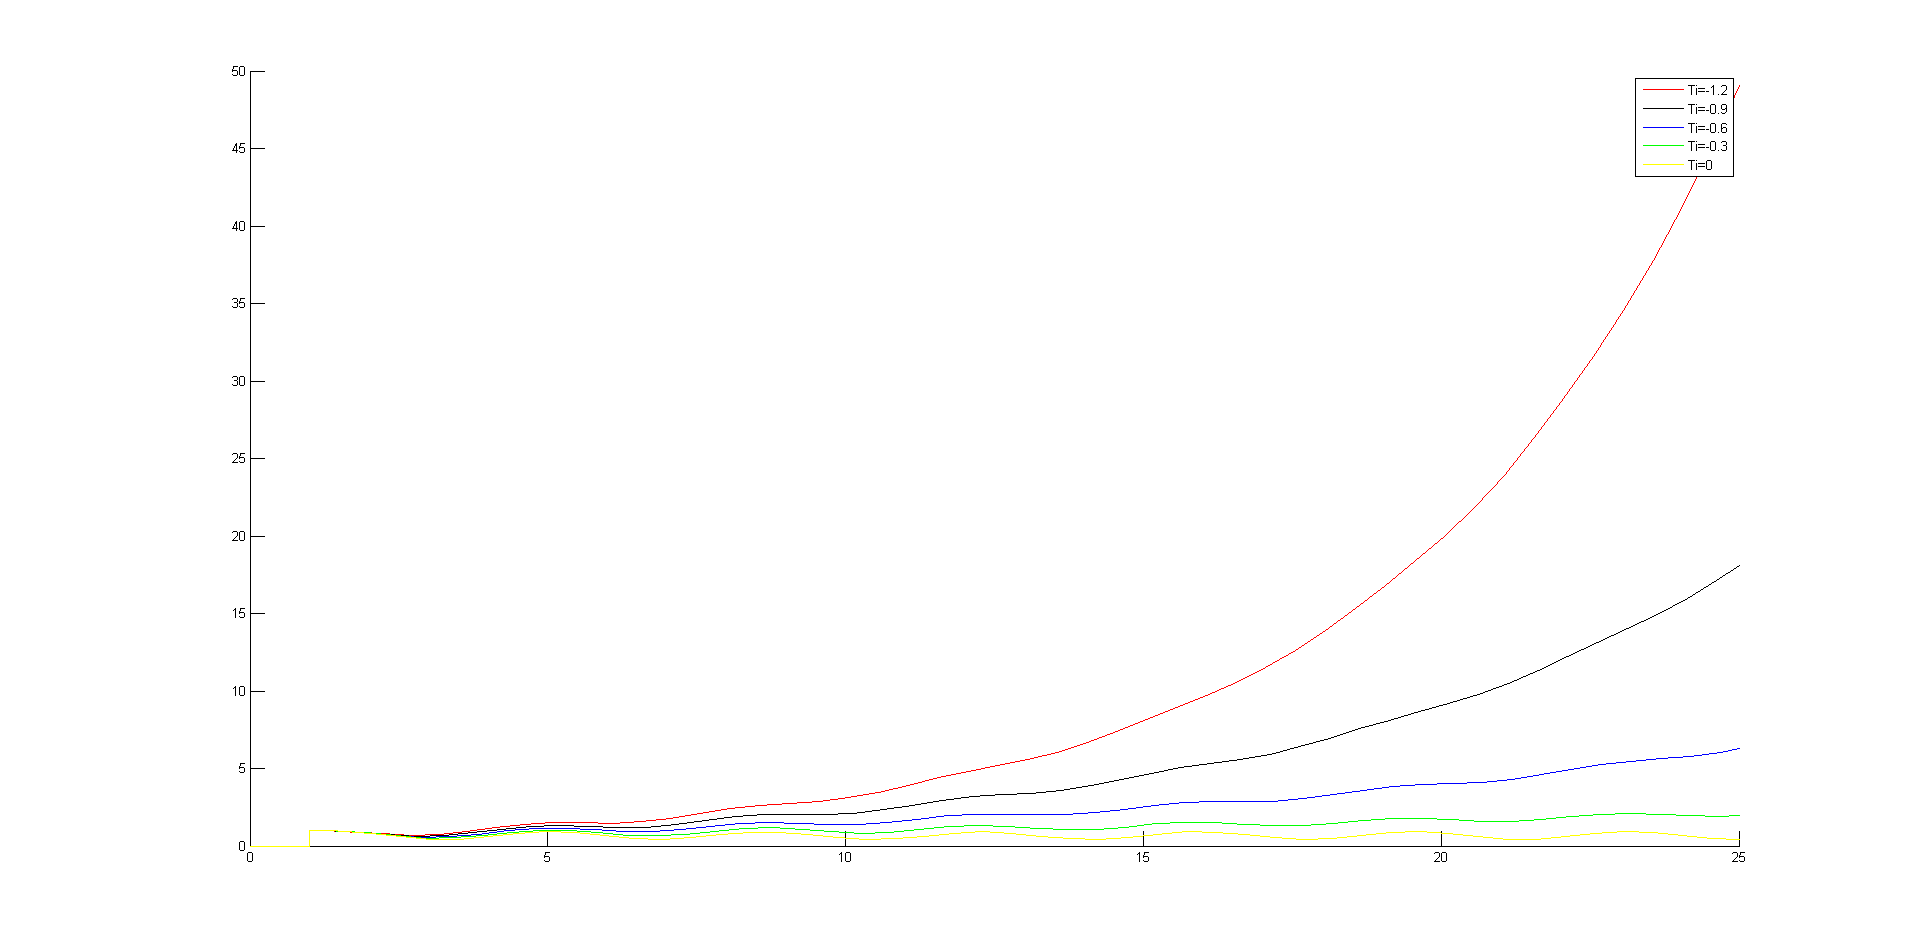
\includegraphics[width=130mm]{CW2-regulatorPI-eu.png}
	\caption{Wykres przebiegu funkcji $\varepsilon(t)$ regulatora PI dla wartości ujemnych $T_{i}$.}
    \label{fig:regulatorPIeu}
\end{figure}
\begin{figure}[!h]
    \centering
	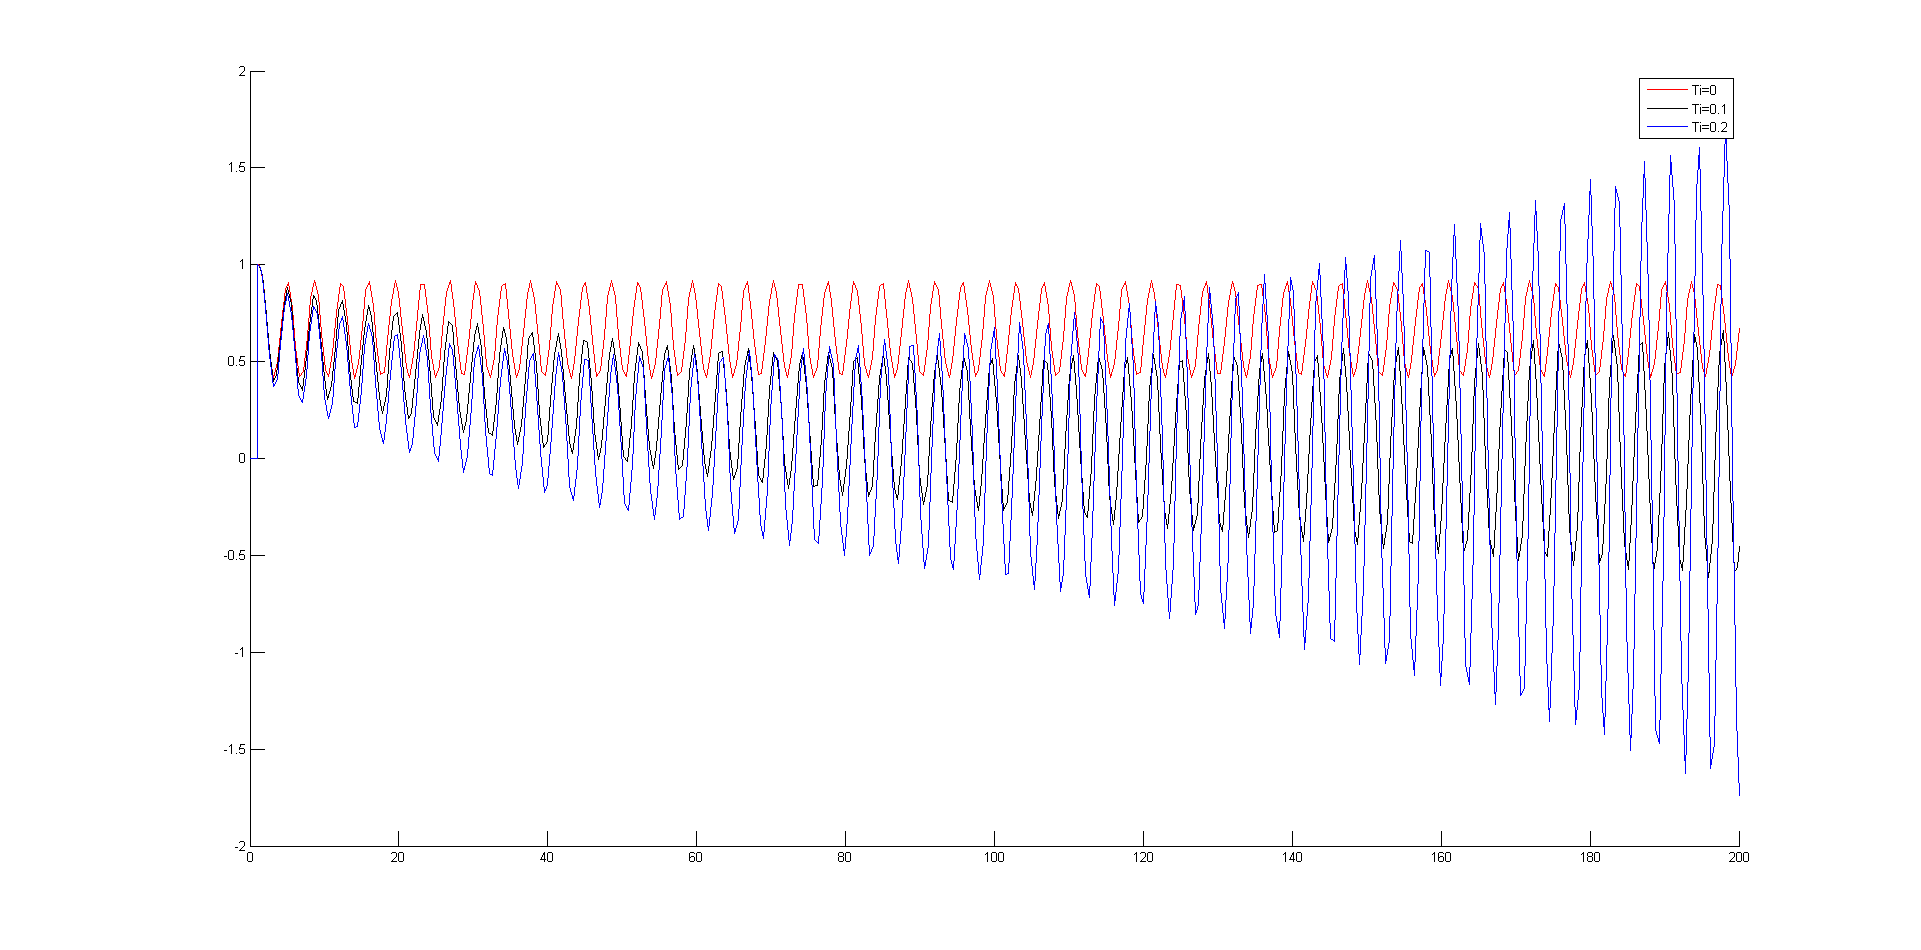
\includegraphics[width=130mm]{CW2-regulatorPI-ed.png}
	\caption{Wykres przebiegu funkcji $\varepsilon(t)$ regulatora PI dla wartości dodatnich $T_{i}$.}
    \label{fig:regulatorPIed}
\end{figure}
\newpage Z wykresu \ref{fig:regulatorPIeu}, oraz \ref{fig:regulatorPIed} możemy zauważyć, że:
\begin{itemize}
	\item Dla ujemnych wartości parametru $T_{i}$ wartości funkcji $\varepsilon(t)$ szybko rosną. Tempo w jakim wzrasta jest tym większe im mniejszą wartość ma parametr $T_{i}$.
	\item Dla wartości dodatnich wykres $\varepsilon(t)$ przyjmuje postać drgań, które z początku oscylują tak jak przy regulatorze P, lecz z czasem oscylują wokół wartości coraz bliższej 0. Tempo w jakim zbliża się do 0 jest tym większe im większą wartość ma parametr $T_{i}$. Amplituda drgań z czasem wzrasta.
	\item Regulator PI jest bardziej efektywny niż regulator P, ponieważ wykres funkcji $\varepsilon(t)$ oscyluje bliżej 0.
\end{itemize}
\subsubsection{Regulator PID.}\label{sec:regPID}
Aby zasymulować regulator P musieliśmy ustawić wartości parametru proporcjonalnego i całkujacego na $k=2$, $T_{i}=1$. \\
Następnie wykorzystując poniższą funkcję przetestowaliśmy zachowanie regulatora P dla różnych wartości parametru $T_{d}$. \\
\begin{lstlisting}[caption=Funkcja testująca regulator P.]
function testPID(start, step, stop)
load_system('model.mdl');
hold on;
td = start;
color = char('r', 'k', 'b', 'g', 'y', 'm');
set_param('model/Gain', 'Gain', num2str(2));
set_param('model/Gain1', 'Gain', num2str(1));
while (td <= stop)
    set_param('model/Gain2', 'Gain', num2str(td));
    sim('model.mdl');
    wy = simout.signals.values;
    figure(1);
    plot(tout, wy, 'Color', color(mod(i,6)+1));
    td = td + step;
end
end
\end{lstlisting}
W ten sposób otrzymalismy następujące wykresy: \\
\begin{figure}[!h]
    \centering
	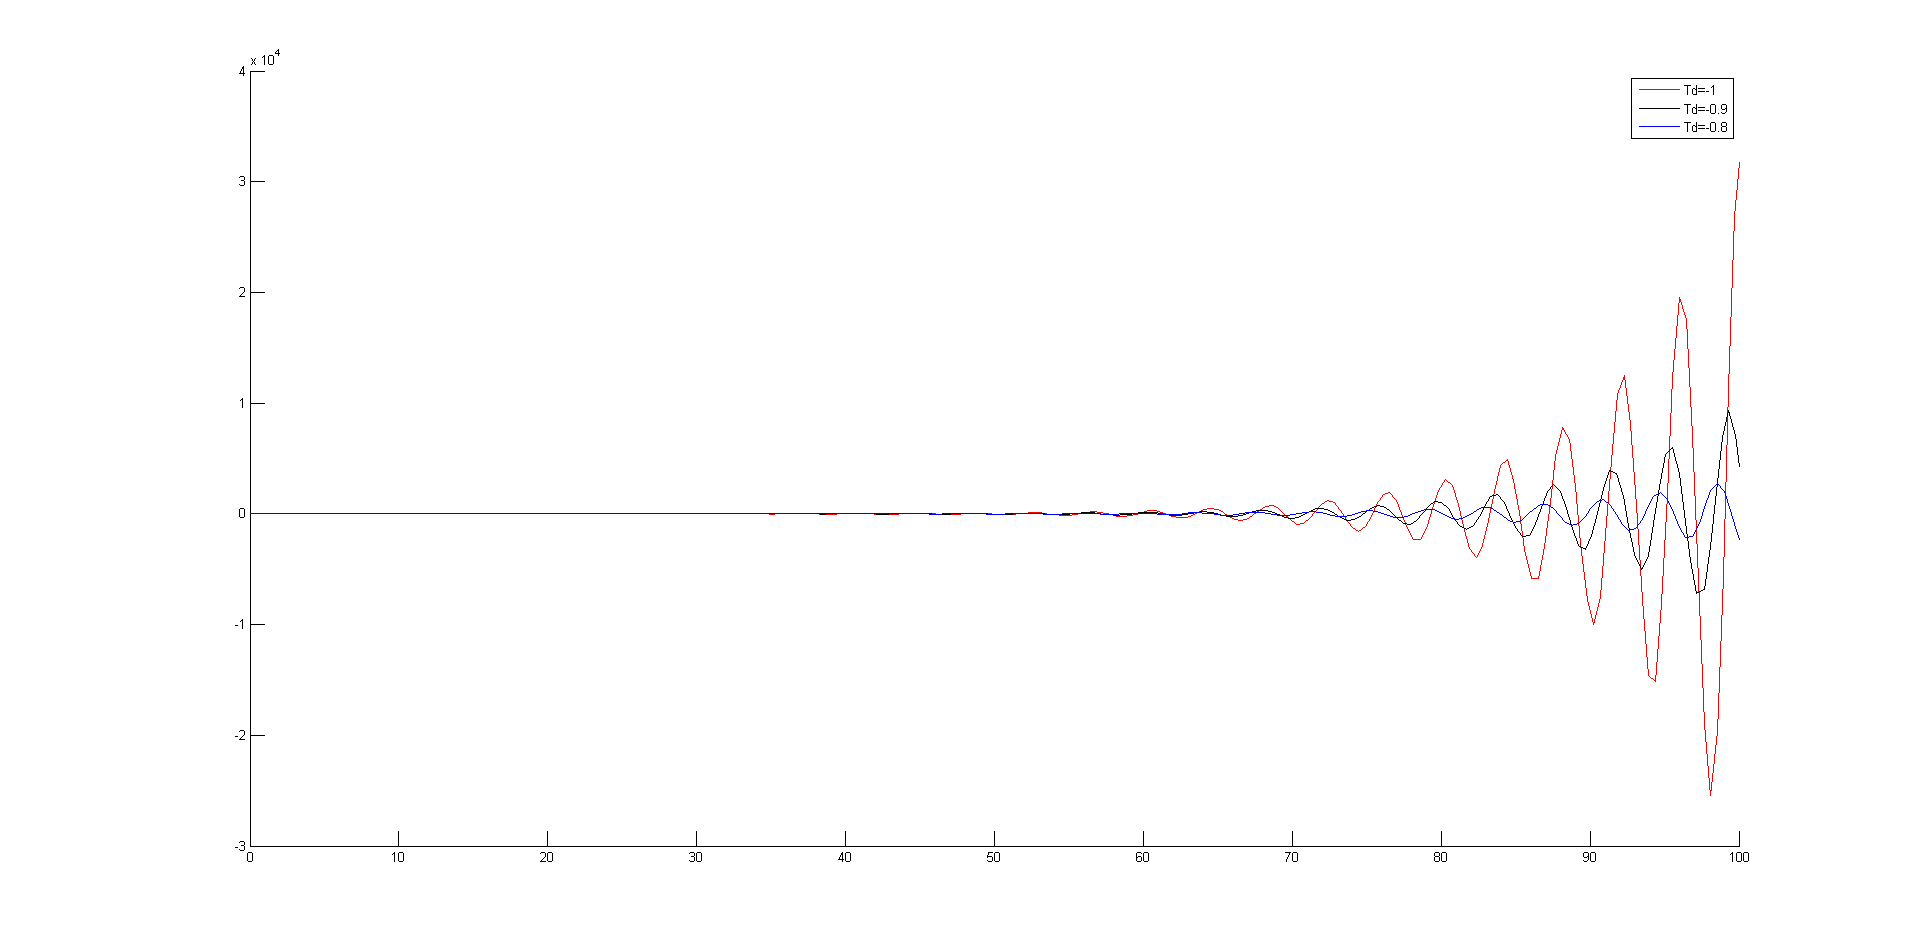
\includegraphics[width=130mm]{CW2-regulatorPID-eu.png}
	\caption{Wykres przebiegu funkcji $\varepsilon(t)$ regulatora PID dla wartości ujemnych $T_{d}$.}
    \label{fig:regulatorPIDeu}
\end{figure}
\begin{figure}[!h]
    \centering
	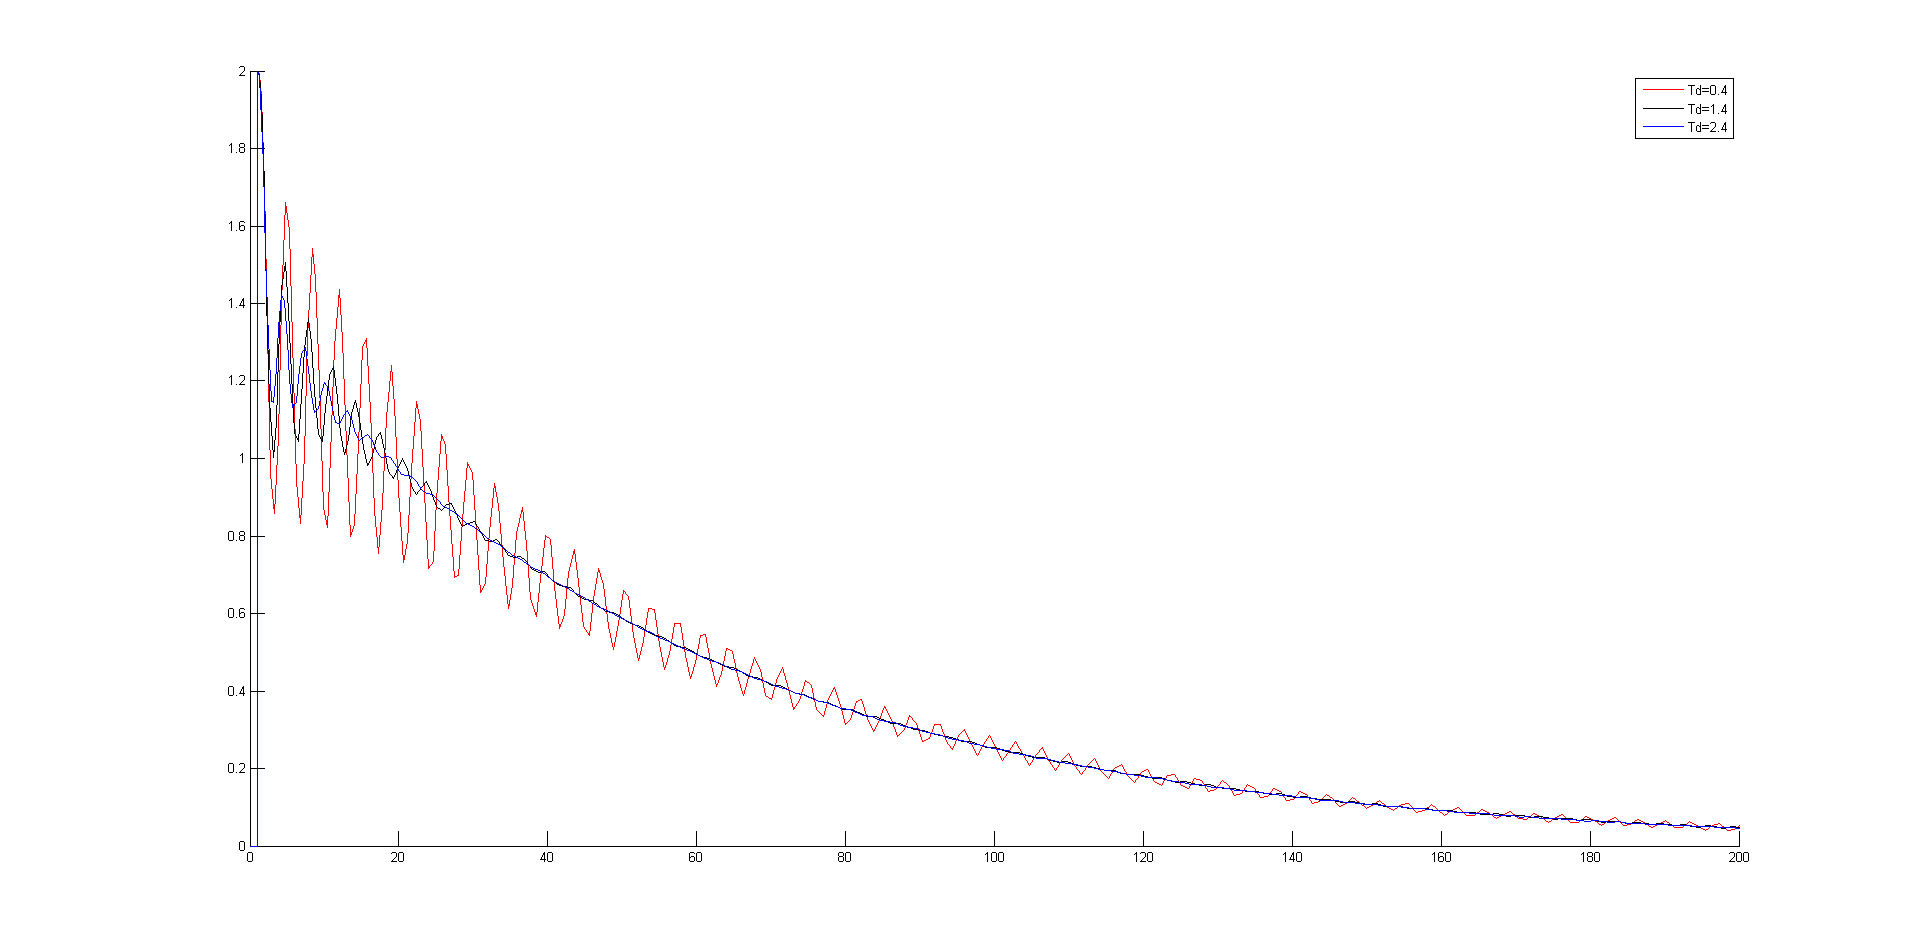
\includegraphics[width=130mm]{CW2-regulatorPID-ed.png}
	\caption{Wykres przebiegu funkcji $\varepsilon(t)$ regulatora PID dla wartości dodatnich $T_{d}$.}
    \label{fig:regulatorPIDed}
\end{figure}
\newpage Z wykresu \ref{fig:regulatorPIDeu}, oraz \ref{fig:regulatorPIDed} możemy zauważyć, że:
\begin{itemize}
	\item Dla ujemnych wartości parametru $k$ wykres $\varepsilon(t)$ przyjmuje postać drgań, których amplituda z czasem rośnie. Tempo tego wzrostu jest tym większe im mniejszą wartość ma parametr $T_{d}$.
	\item Dla wartości dodatnich wykres $\varepsilon(t)$ przyjmuje postać drgań, które oscylują tak jak przy regulatorze PI, lecz z czasem amplituda maleje. Tempo w jakim ona maleje tym większe im większą wartość ma parametr $T_{d}$.
	\item Regulator PID jest efektywny, ponieważ wykres funkcji $\varepsilon(t)$ oscyluje bliżej 0 niż regulator P, a amplituda drgań, która w regulatorze PI się zwiększała tutaj zanika.
\end{itemize}

%---------------------------------------------------------------------------------------------------------------------
%
%ZADANIE 2
%
%---------------------------------------------------------------------------------------------------------------------
\subsection{Dobór optymalnych parametrów regulatora.}\label{sec:zad2}
Przy doborze optymalnych parametrów przyjęliśmy następujące kryterium:
\begin{equation} \label{eqn:transOS}
	Q = {1 \over n}\sum_{i=1}^{n} \varepsilon(t)
\end{equation}
Gdzie $n$ jest ilością pomiarów wykonanych przy symulacji.

\subsubsection{Regulator P.}\label{sec:optP}
Aby dobrać optymalną wartość parametru $k$ ustawiliśmy parametry podobnie jak w zadaniu \ref{sec:regP}, oraz wykorzystując poniższą funkcję przetestowaliśmy zachowanie regulatora P dla wielu wartości parametru $k$. \\
\newpage \begin{lstlisting}[caption=Funkcja testująca regulator P.]
function optimumP(start, step, stop)
load_system('model.mdl');
hold on;
k = start;
i = 0;
set_param('model/Gain1', 'Gain', num2str(0));
set_param('model/Gain2', 'Gain', num2str(0));
while (k <= stop)
    set_param('model/Gain', 'Gain', num2str(k));
    sim('model.mdl');
    wy = simout.signals.values;
    i = i + 1;
    q(i) = sum(wy.^2)/length(wy);
    ka(i) = k;
    k = k + step;
end
figure(1);
plot(ka, q);
end
\end{lstlisting}
W ten sposób otrzymalismy następujące wykresy: \\
\begin{figure}[!h]
    \centering
	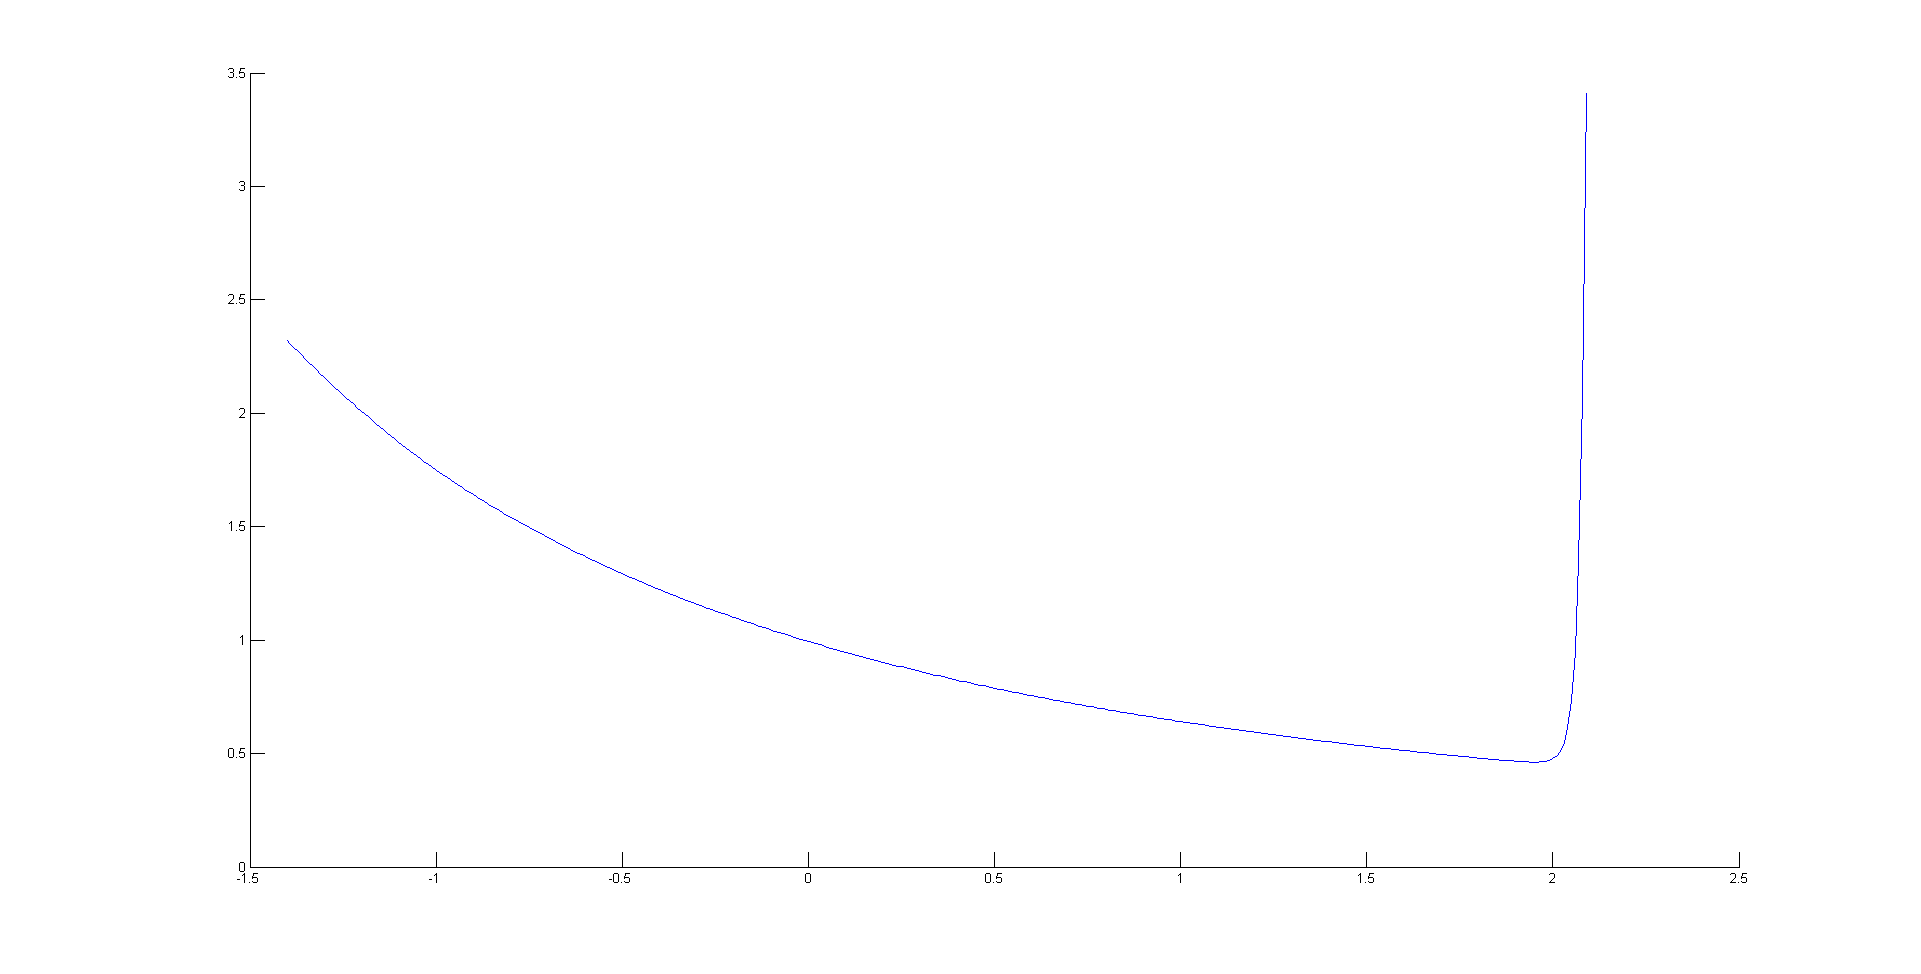
\includegraphics[width=130mm]{CW2-regulatorP-opt1.png}
	\caption{Wykres przebiegu funkcji $Q(k)$ regulatora P.}
    \label{fig:regulatorPopt1}
\end{figure}
\begin{figure}[!h]
    \centering
	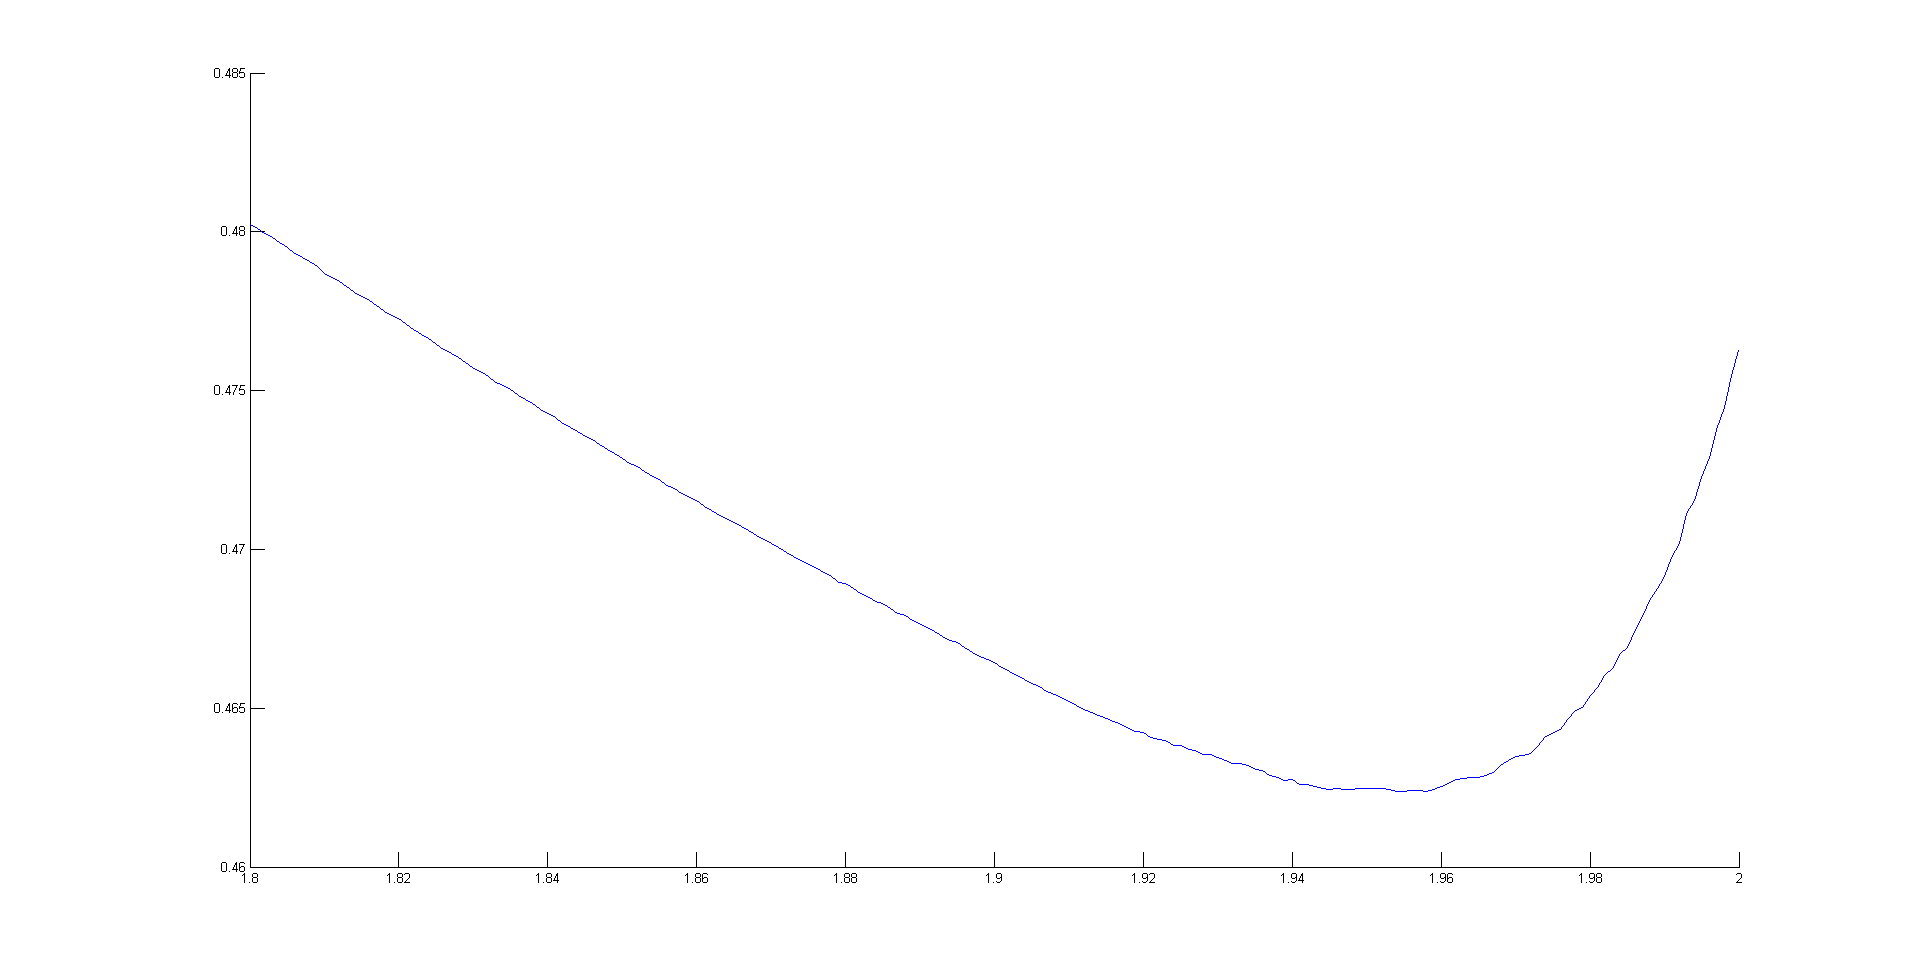
\includegraphics[width=130mm]{CW2-regulatorP-opt2.png}
	\caption{Wykres przebiegu funkcji $Q(k)$ regulatora P (powiększenie).}
    \label{fig:regulatorPopt2}
\end{figure}
\\ Wartością optymalną parametru $k$ jest minimum funkcji $Q(k)$, więc z wykresu \ref{fig:regulatorPopt1}, oraz \ref{fig:regulatorPopt2} możemy odczytać, że $k \approx 1.95$.

\subsubsection{Regulator PI.}\label{sec:optPI}
Aby dobrać optymalną wartość parametru $T_{i}$ ustawiliśmy parametry podobnie jak w zadaniu \ref{sec:regPI}, oraz wykorzystując poniższą funkcję przetestowaliśmy zachowanie regulatora P dla wielu wartości parametru $T_{i}$ i trzech różnych wartości $k$. \\
\begin{lstlisting}[caption=Funkcja testująca regulator P.]
function optimumPI(start, step, stop)
load_system('model.mdl');
hold on;
ti = start;
i = 0;
set_param('model/Gain2', 'Gain', num2str(0));
set_param('model/Gain', 'Gain', num2str(1));
while (ti <= stop)
    set_param('model/Gain1', 'Gain', num2str(ti));
    sim('model.mdl');
    wy = simout.signals.values;
    i = i + 1;
    q(i) = sum(wy.^2)/length(wy);
    tei(i) = ti;
    ti = ti + step;
end
figure(1);
plot(tei, q);
end
\end{lstlisting}
W ten sposób otrzymalismy następujące wykresy: \\
\begin{figure}[!h]
    \centering
	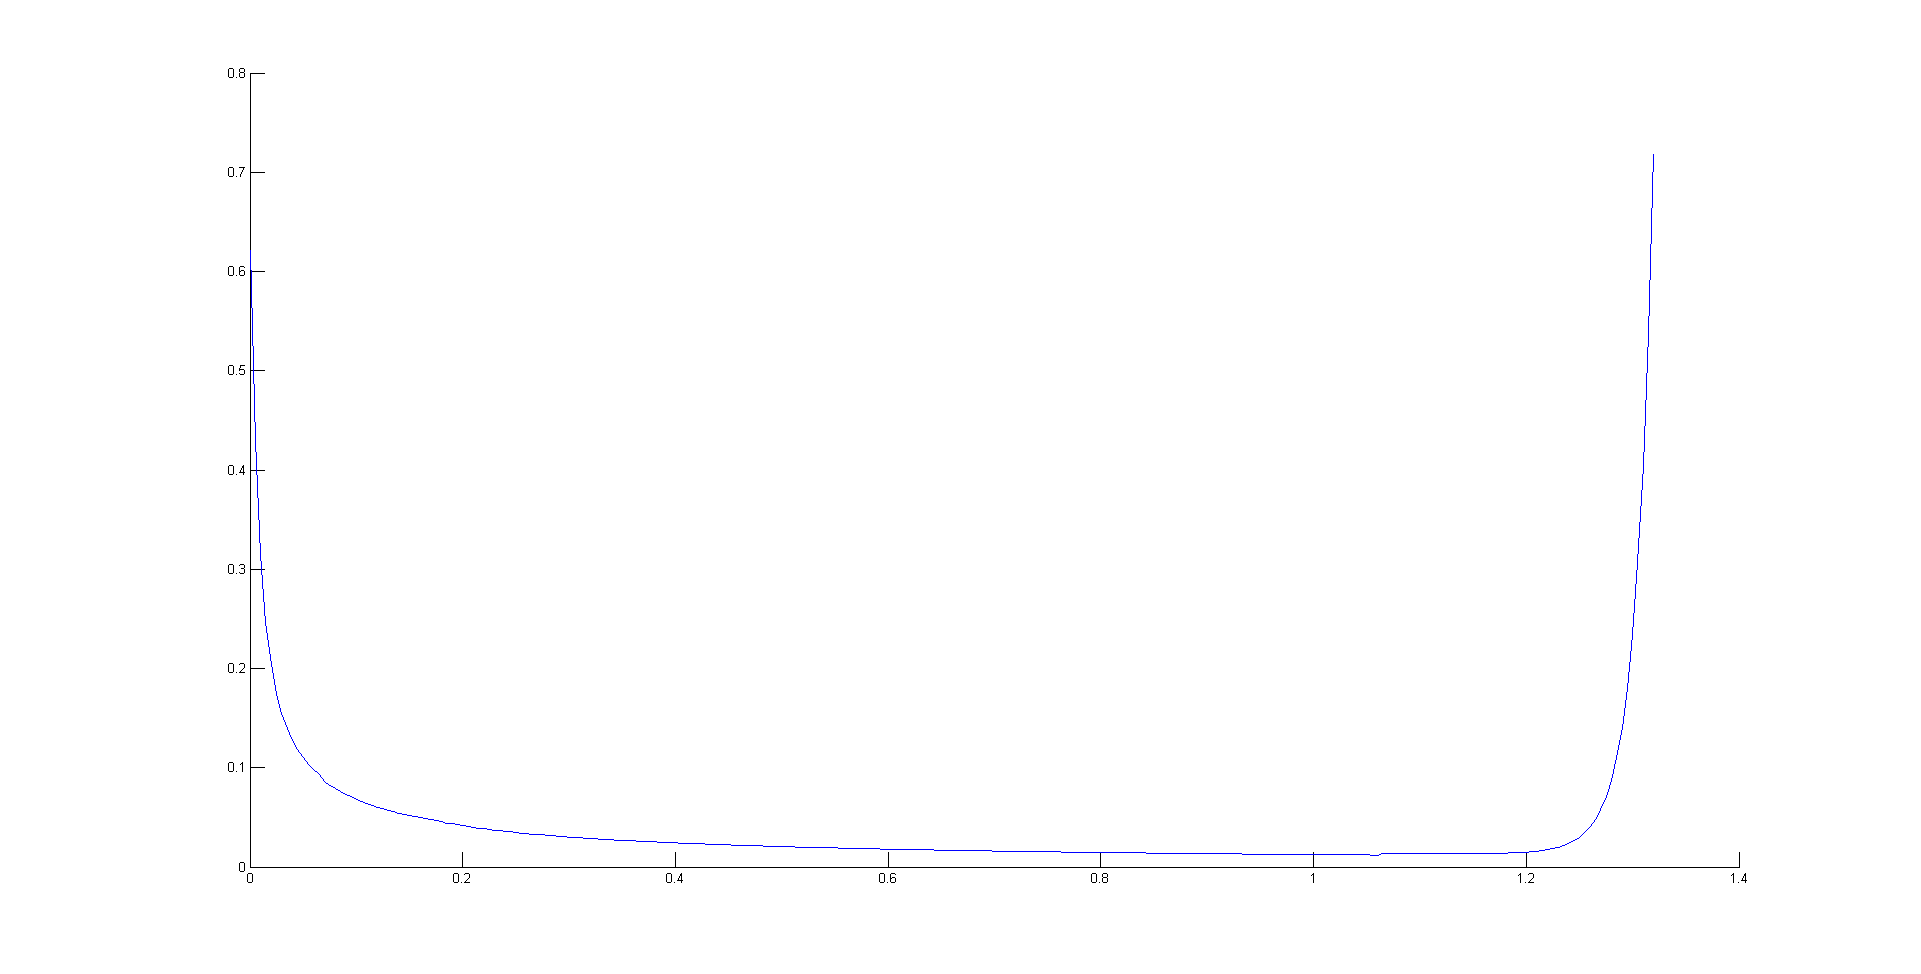
\includegraphics[width=130mm]{CW2-regulatorPI-k1-opt1.png}
	\caption{Wykres przebiegu funkcji $Q(T_{i})$ regulatora P dla $k=1$.}
    \label{fig:regulatorPIk1opt1}
\end{figure}
\begin{figure}[!h]
    \centering
	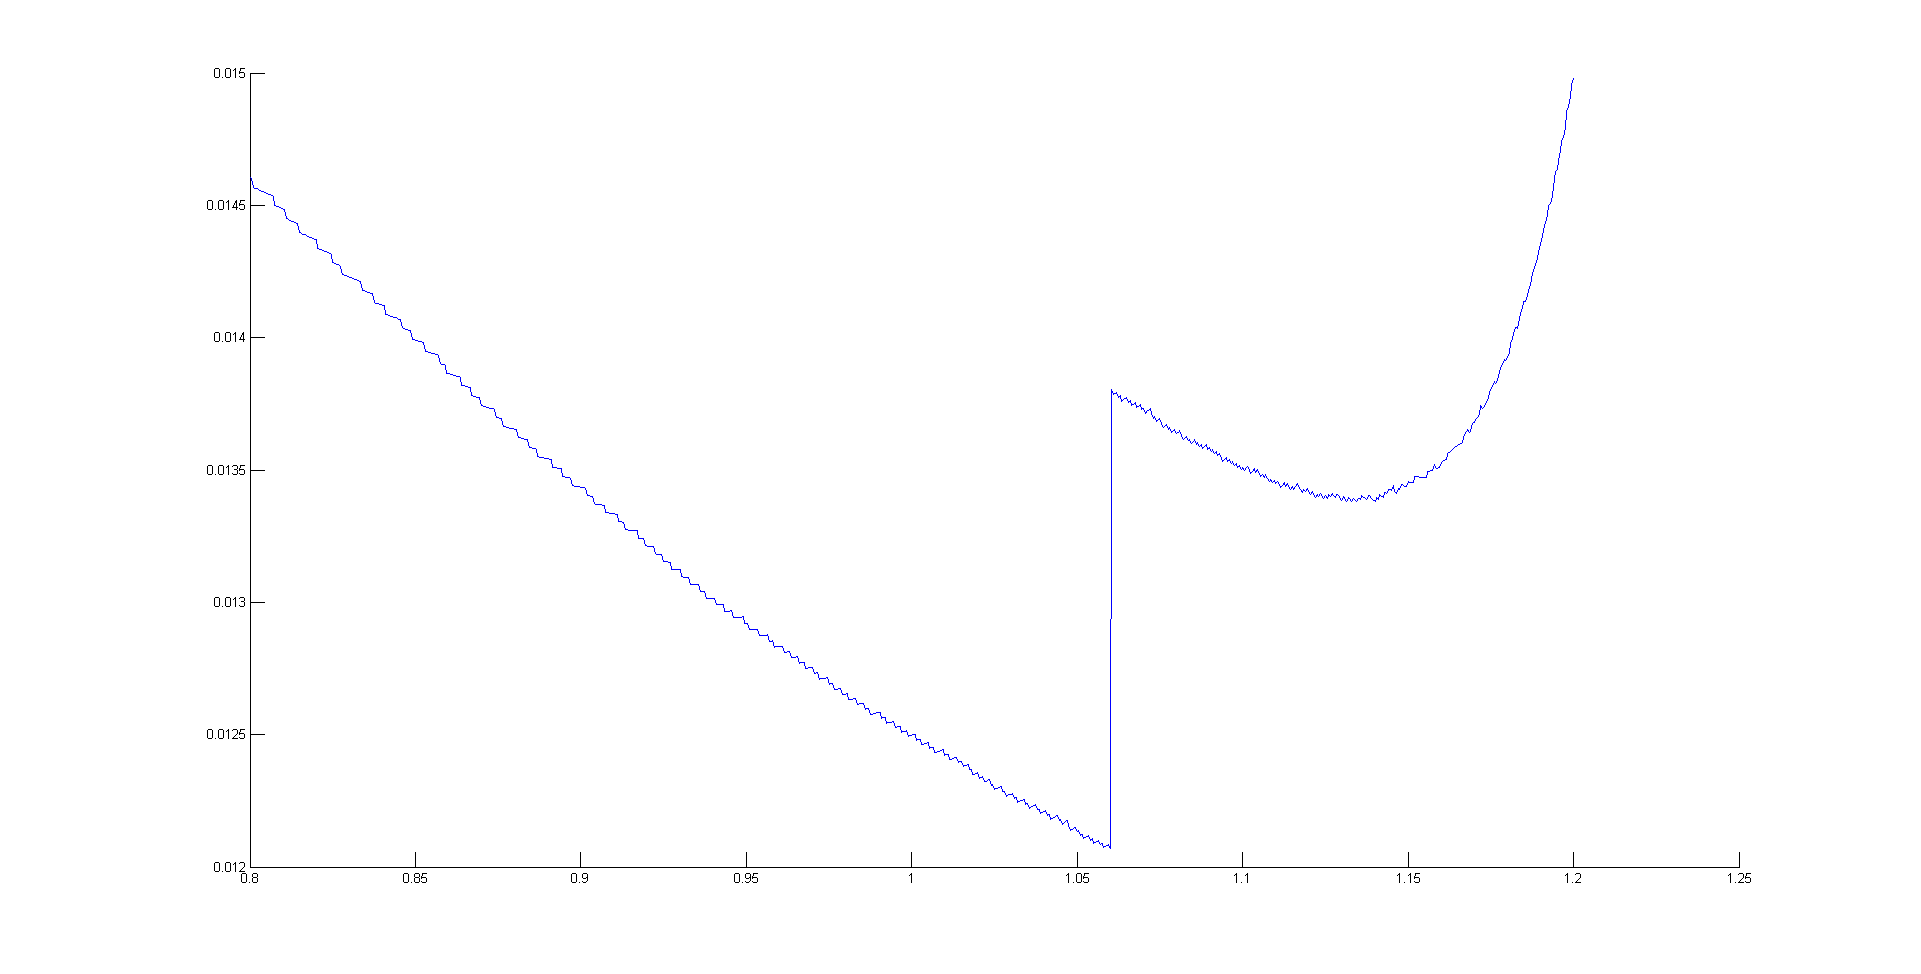
\includegraphics[width=130mm]{CW2-regulatorPI-k1-opt2.png}
	\caption{Wykres przebiegu funkcji $Q(T_{i})$ regulatora P dla $k=1$ (powiększenie).}
    \label{fig:regulatorPIk1opt2}
\end{figure}
\begin{figure}[!h]
    \centering
	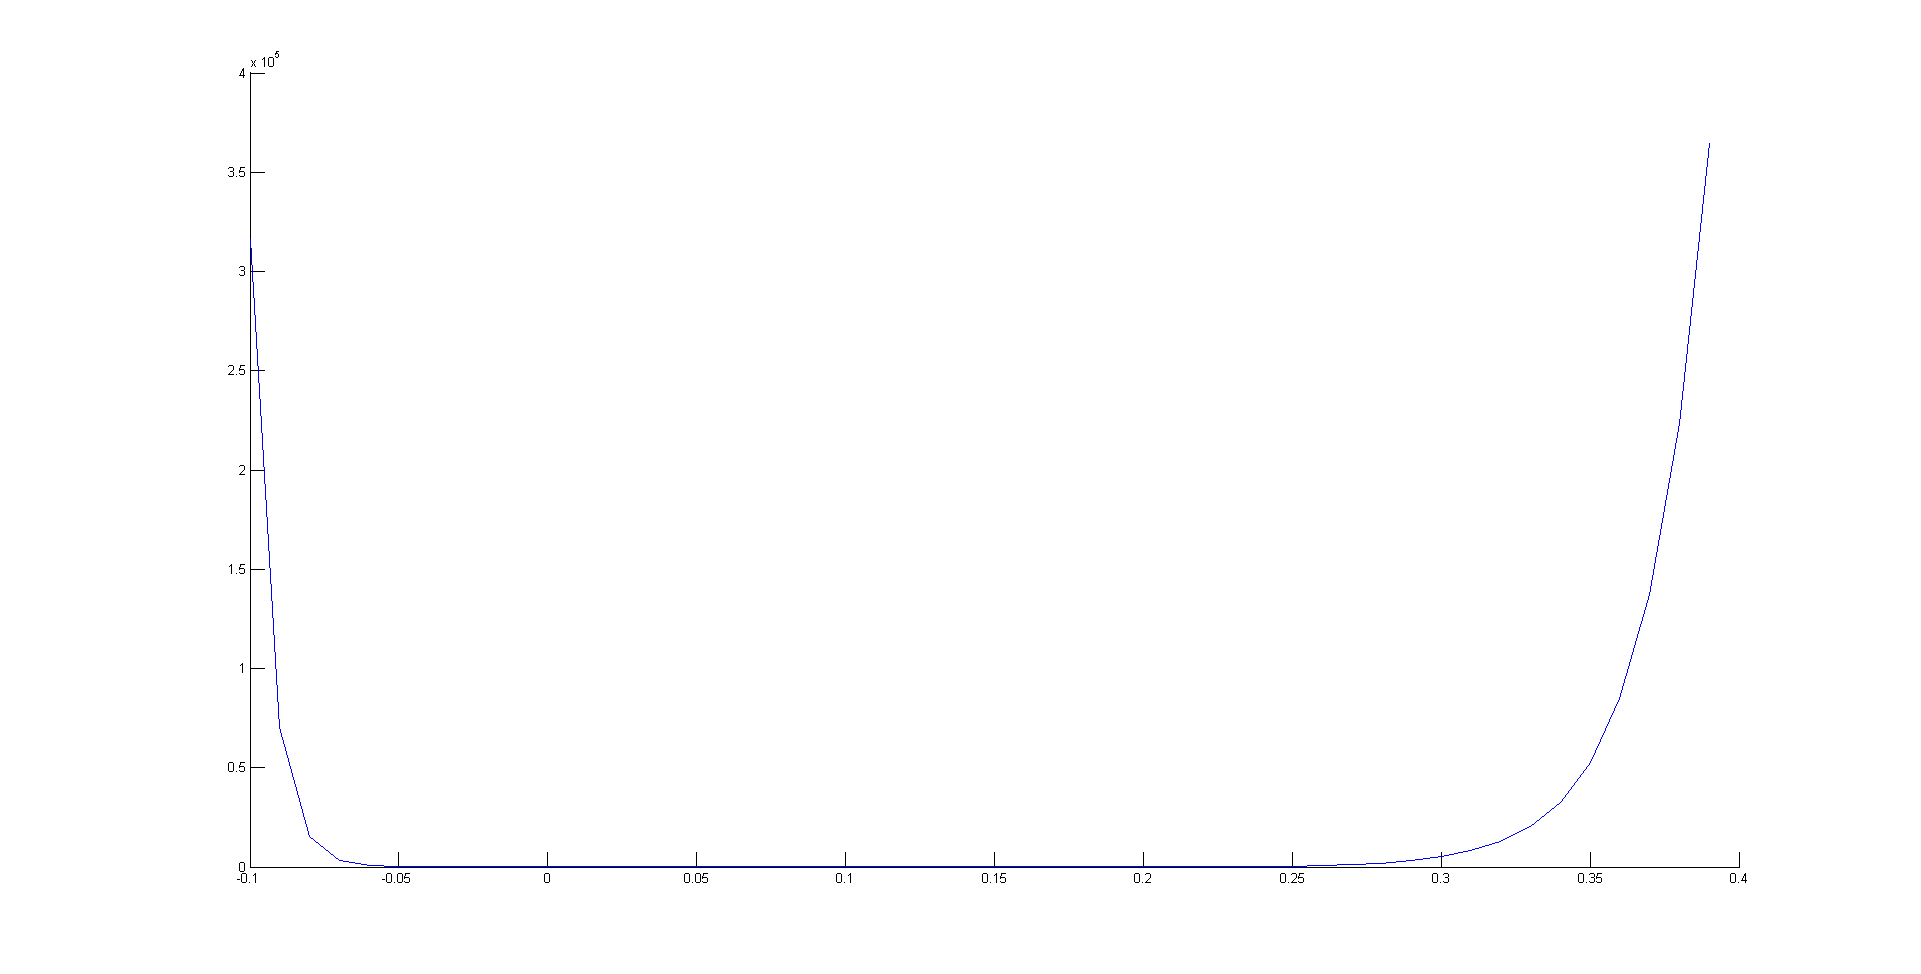
\includegraphics[width=130mm]{CW2-regulatorPI-k2-opt1.png}
	\caption{Wykres przebiegu funkcji $Q(T_{i})$ regulatora P dla $k=2$.}
    \label{fig:regulatorPIk2opt1}
\end{figure}
\begin{figure}[!h]
    \centering
	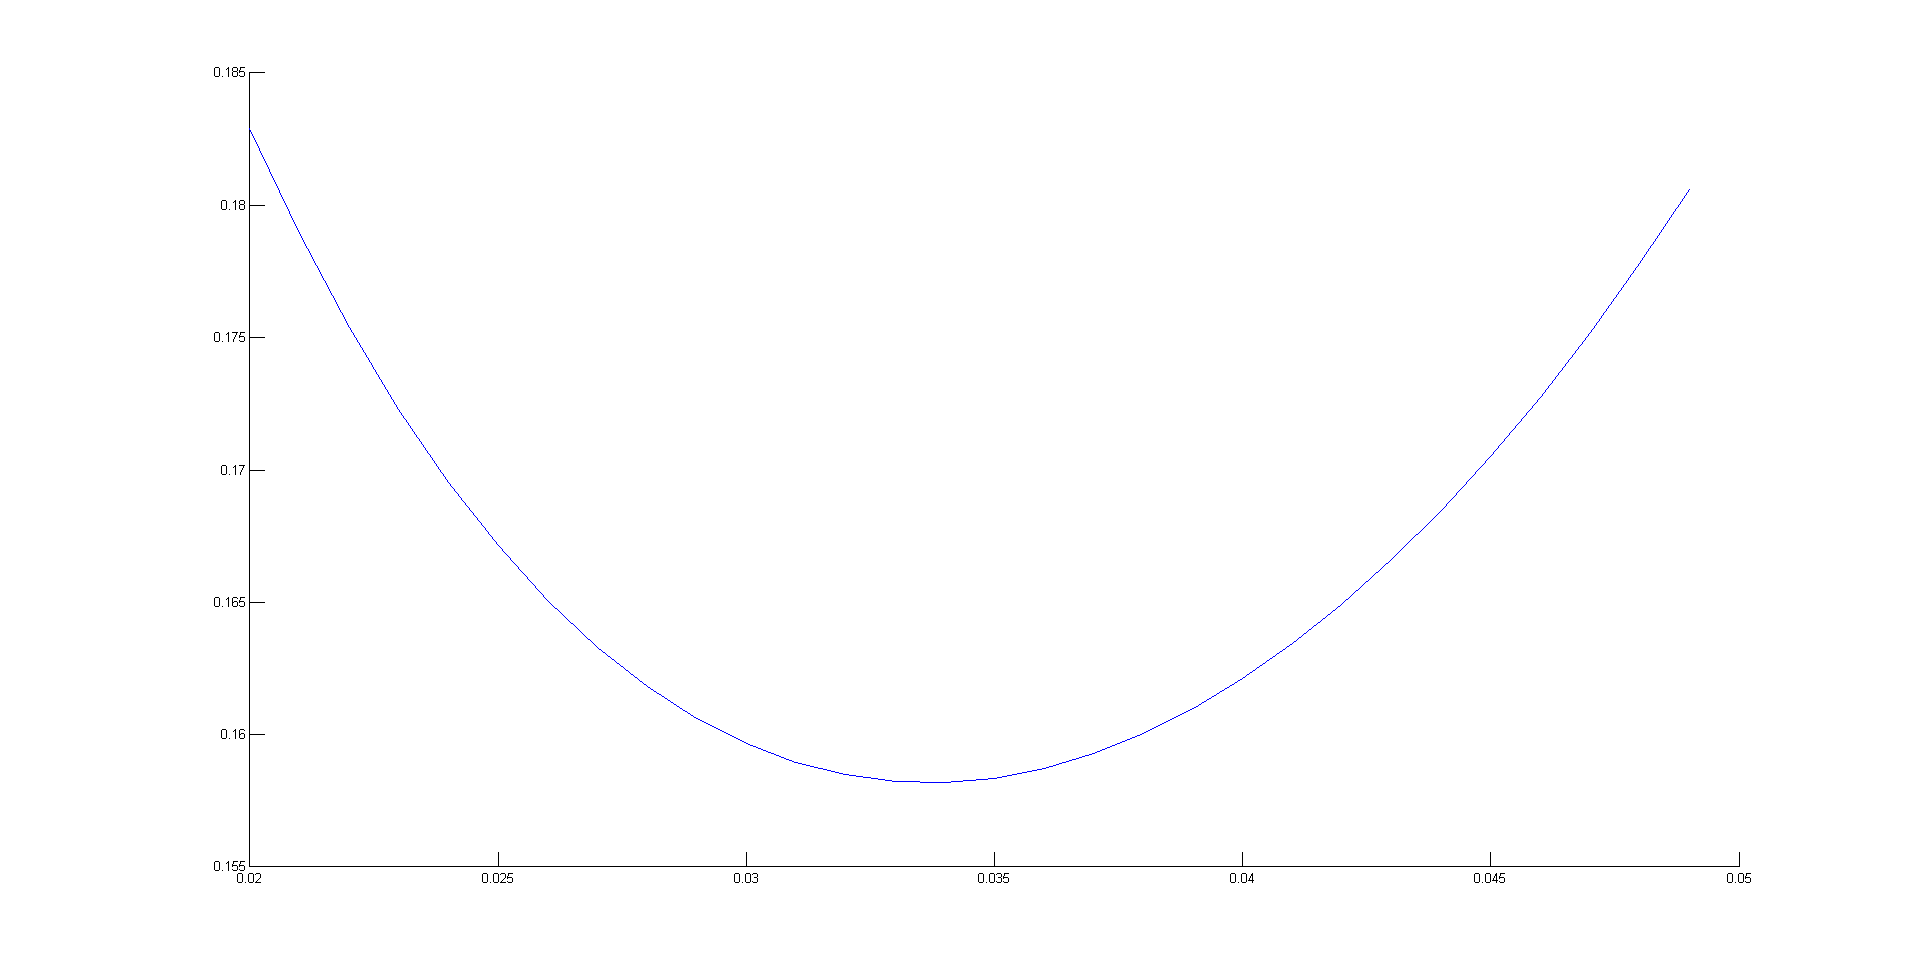
\includegraphics[width=130mm]{CW2-regulatorPI-k2-opt2.png}
	\caption{Wykres przebiegu funkcji $Q(T_{i})$ regulatora P dla $k=2$ (powiększenie).}
    \label{fig:regulatorPIk2opt2}
\end{figure}
\begin{figure}[!h]
    \centering
	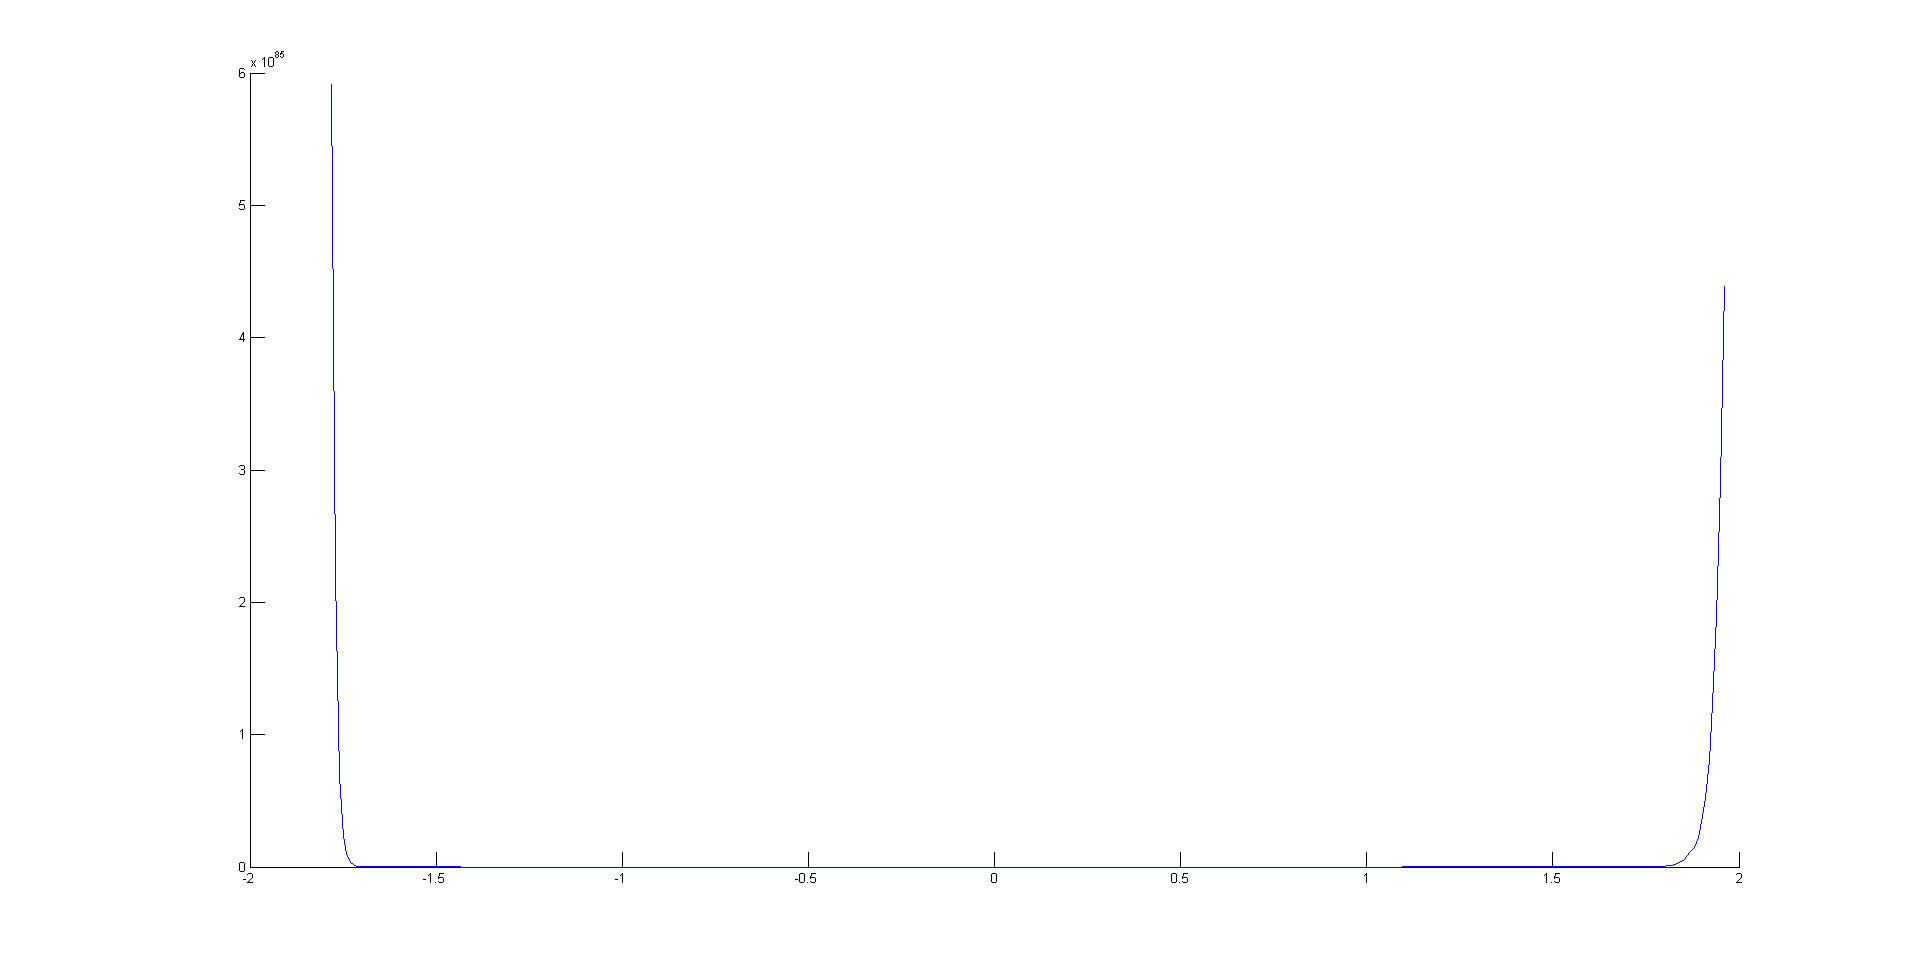
\includegraphics[width=130mm]{CW2-regulatorPI-k4-opt1.png}
	\caption{Wykres przebiegu funkcji $Q(T_{i})$ regulatora P dla $k=4$.}
    \label{fig:regulatorPIk4opt1}
\end{figure}
\begin{figure}[!h]
    \centering
	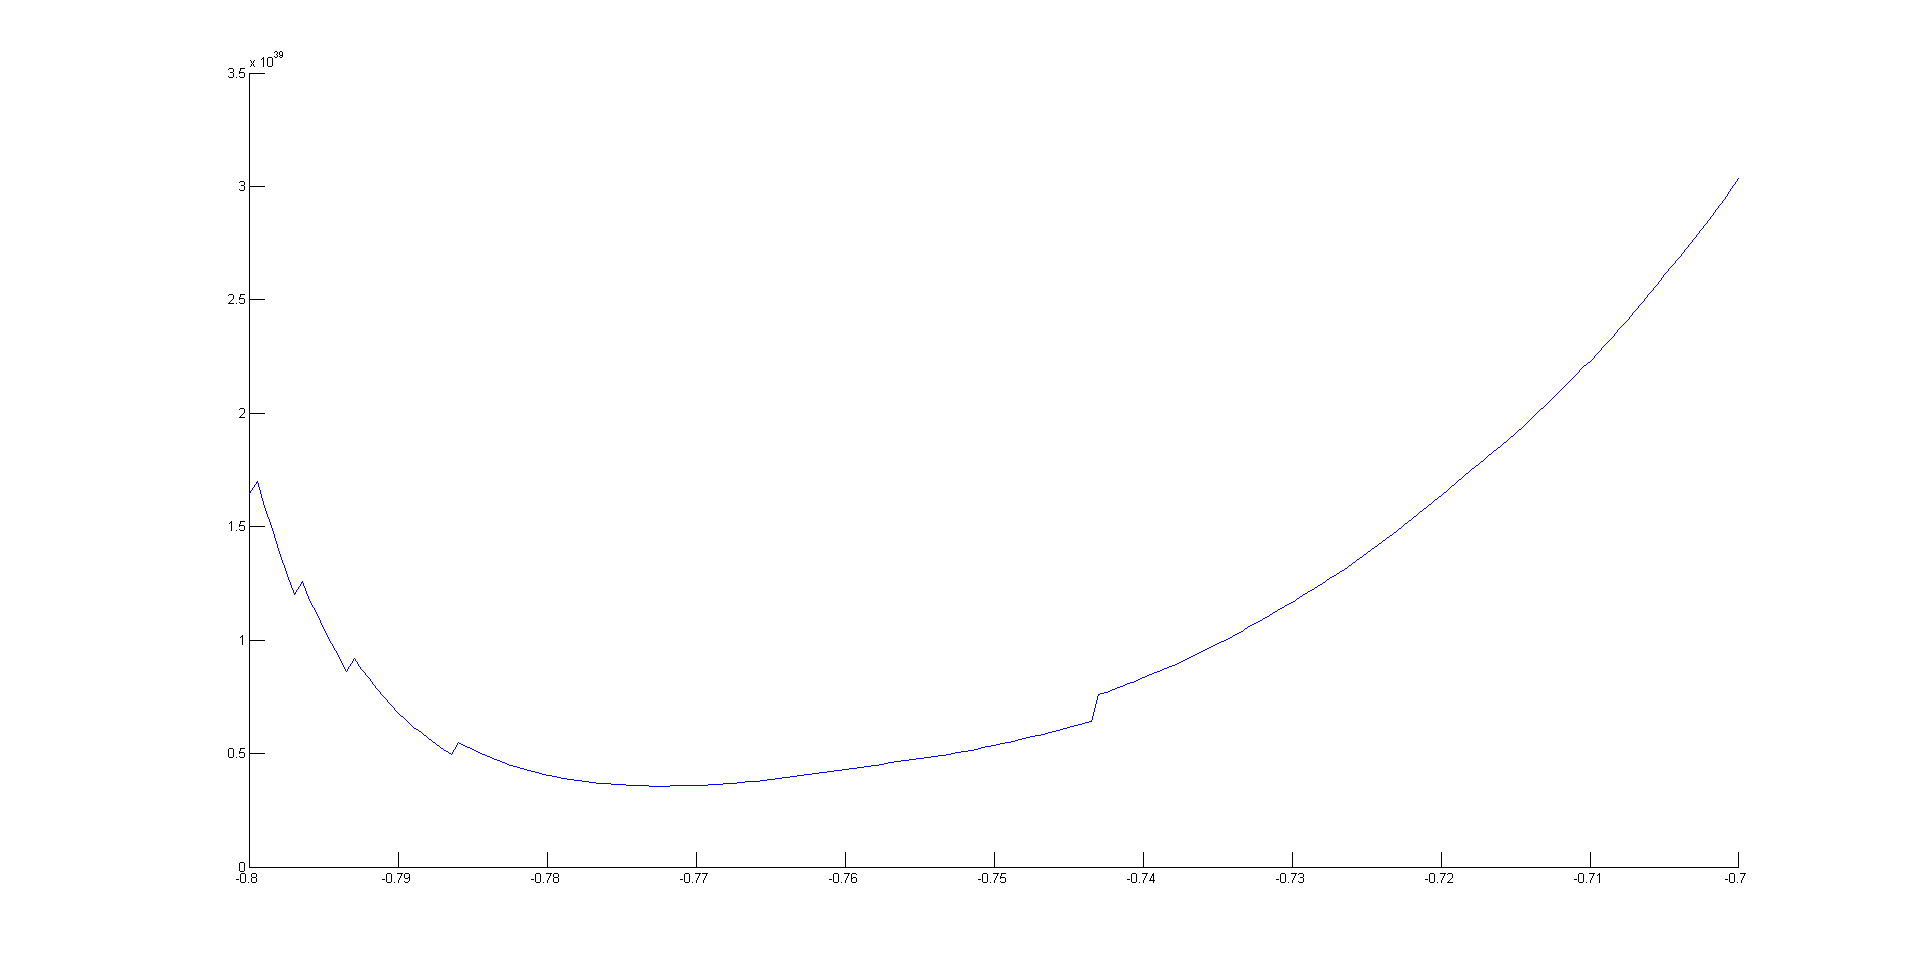
\includegraphics[width=130mm]{CW2-regulatorPI-k4-opt2.png}
	\caption{Wykres przebiegu funkcji $Q(T_{i})$ regulatora P dla $k=4$ (powiększenie).}
    \label{fig:regulatorPIk4opt2}
\end{figure}
\newpage Wartością optymalną parametru $T_{i}$ jest minimum funkcji $Q(T_{i})$, więc z wykresów \ref{fig:regulatorPIk1opt1}, \ref{fig:regulatorPIk1opt2}, \ref{fig:regulatorPIk2opt1}, \ref{fig:regulatorPIk2opt2},\ref{fig:regulatorPIk4opt1}, oraz \ref{fig:regulatorPIk4opt2} możemy odczytać, że dla $k=1, T_{i} \approx 1.05$, dla $k=2, T_{i} \approx 0.35$, natomiast dla $k=4, T_{i} \approx -0.77$.

\subsubsection{Regulator PID.}\label{sec:optPID}
Aby dobrać optymalną wartość parametru $T_{d}$ ustawiliśmy parametry podobnie jak w zadaniu \ref{sec:regPID}, oraz wykorzystując poniższą funkcję przetestowaliśmy zachowanie regulatora P dla wielu wartości parametru $T_{d}$ i trzech różnych wartości $T_{i}$. \\
\newpage \begin{lstlisting}[caption=Funkcja testująca regulator P.]
function testPID(start, step, stop)
load_system('model.mdl');
hold on;
td = start;
i = 0;
set_param('model/Gain', 'Gain', num2str(2));
set_param('model/Gain1', 'Gain', num2str(0.35));
while (td <= stop)
    set_param('model/Gain2', 'Gain', num2str(td));
    sim('model.mdl');
    wy = simout.signals.values;
    i = i + 1;
    q(i) = sum(wy.^2)/length(wy);
    tede(i) = td;
    td = td + step;
end
figure(1);
plot(tede, q);
end
\end{lstlisting}
W ten sposób otrzymalismy następujące wykresy: \\
\begin{figure}[!h]
    \centering
	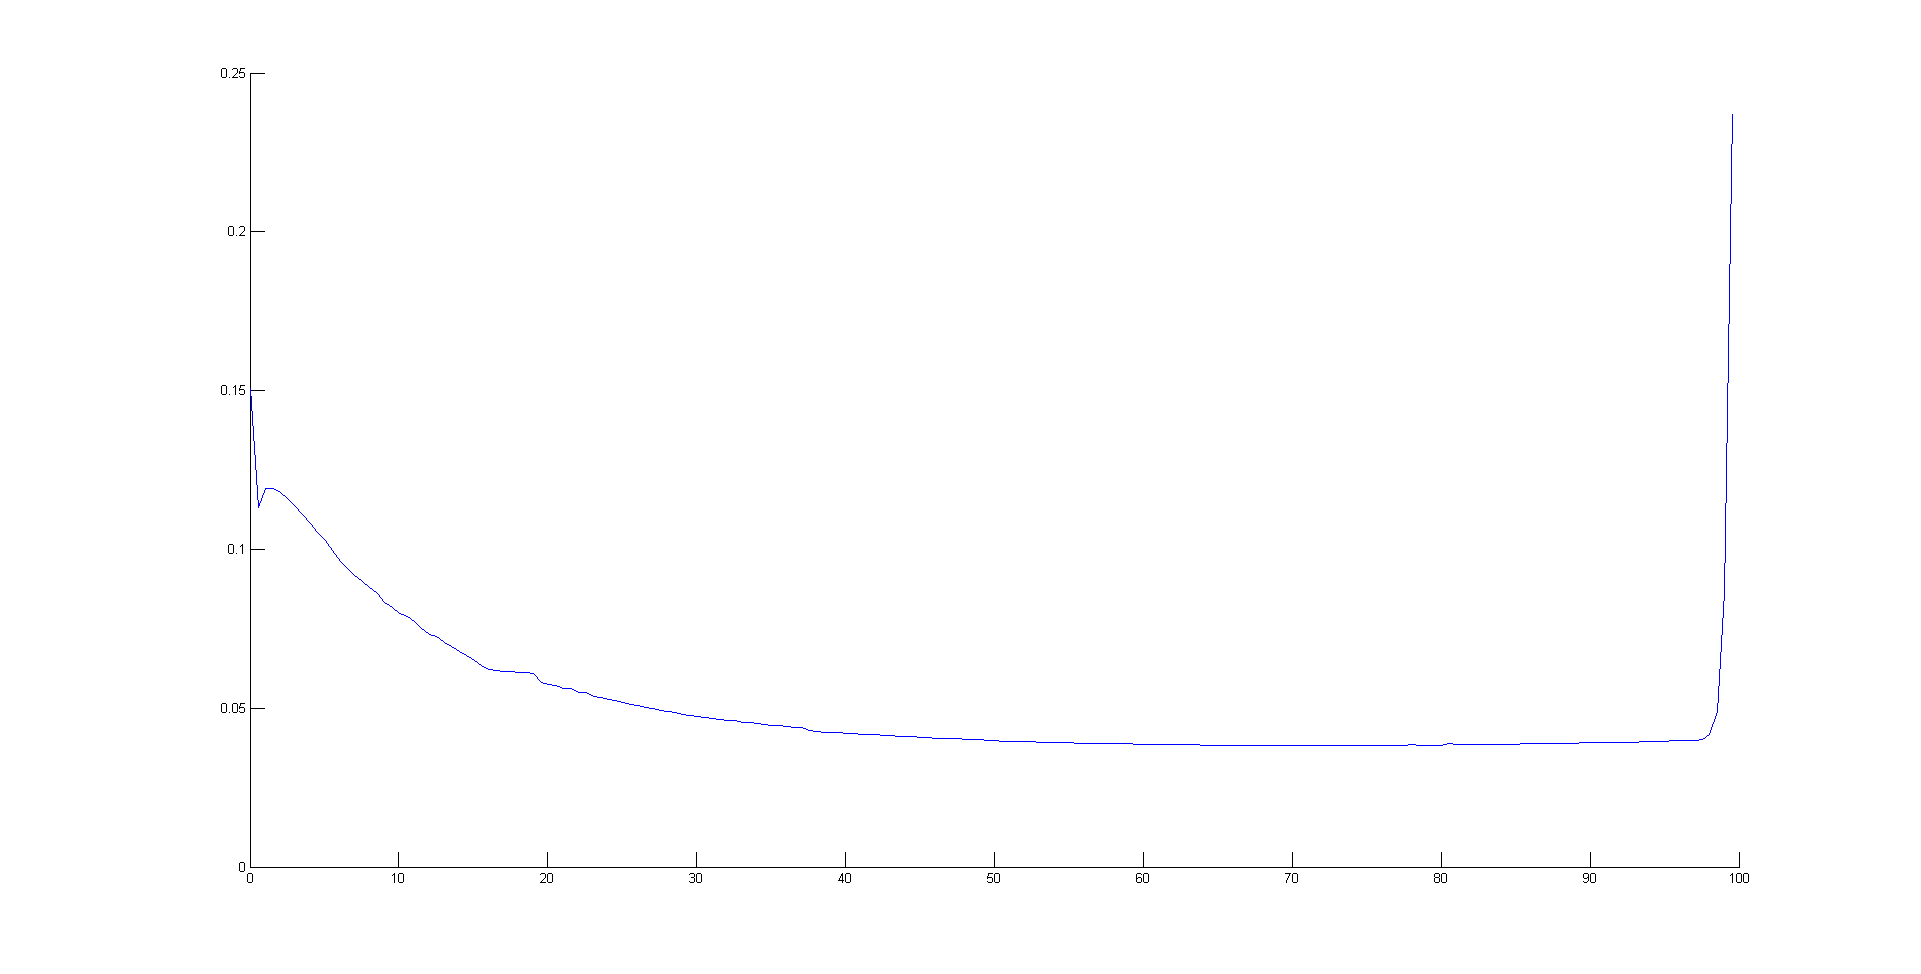
\includegraphics[width=130mm]{CW2-regulatorPID-ti15-opt1.png}
	\caption{Wykres przebiegu funkcji $Q(T_{d})$ regulatora P dla $T_{i}=0.15$.}
    \label{fig:regulatorPIDti15opt1}
\end{figure}
\begin{figure}[!h]
    \centering
	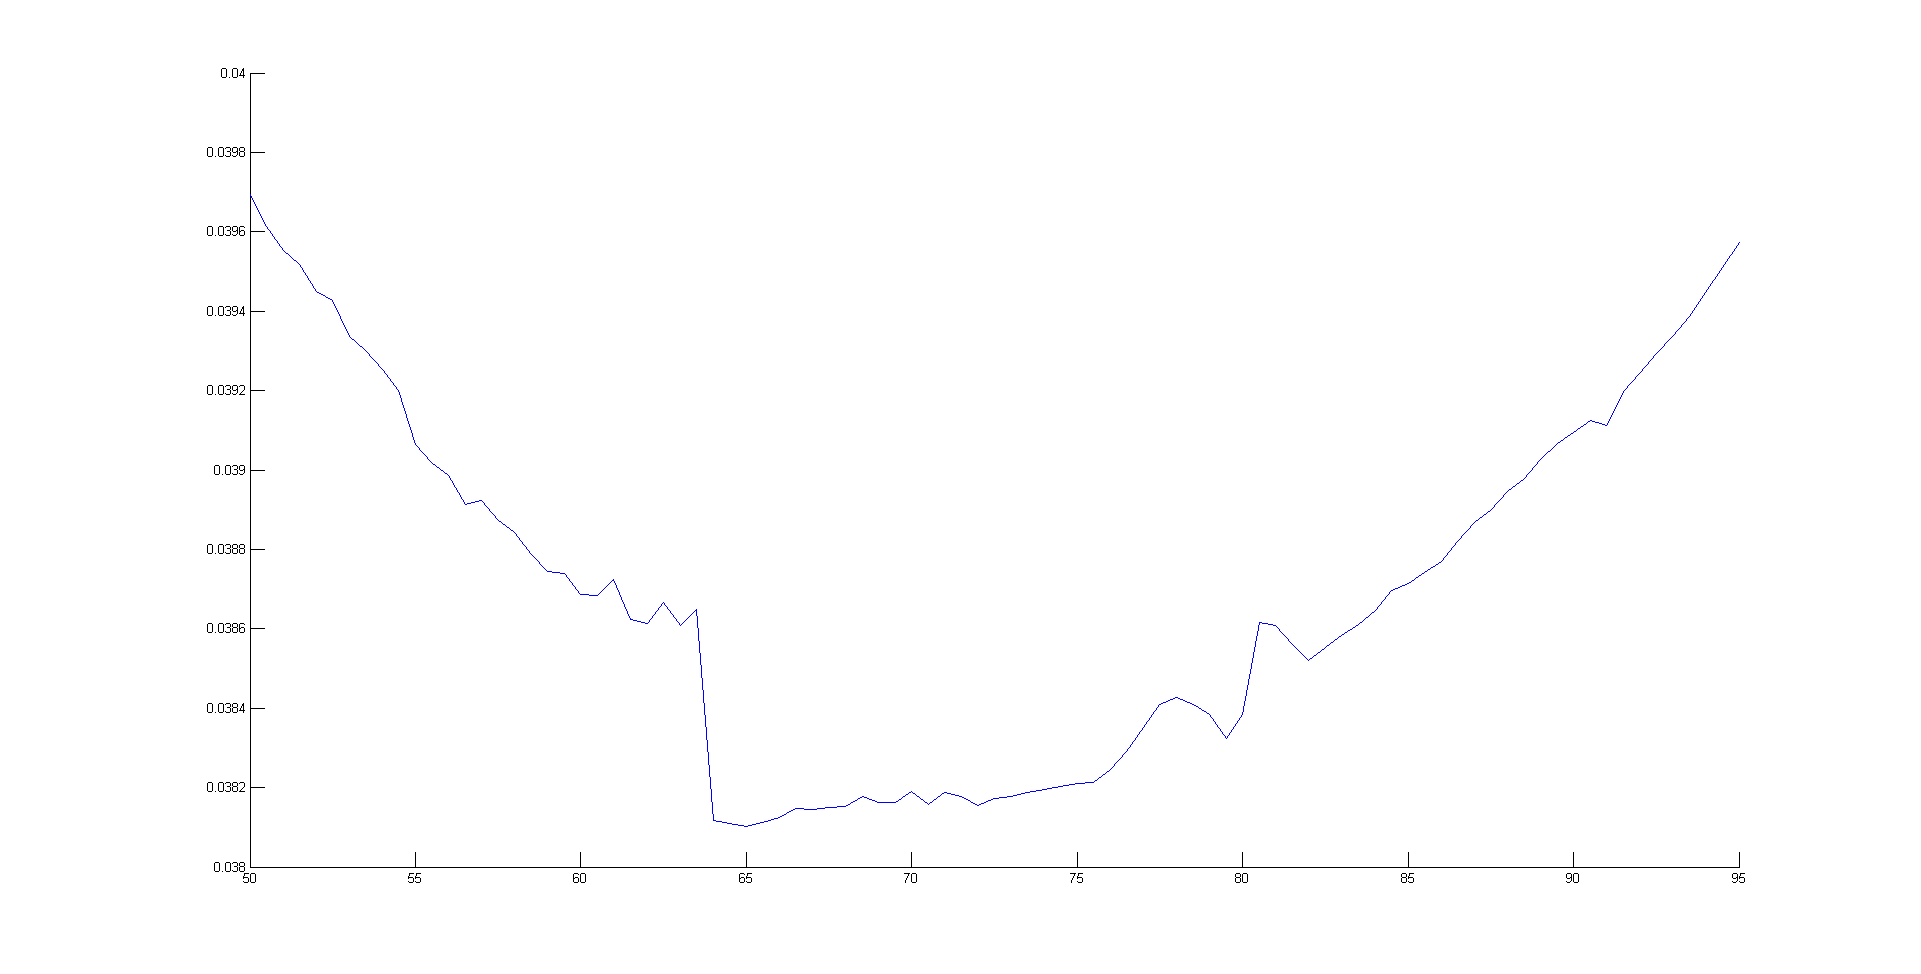
\includegraphics[width=130mm]{CW2-regulatorPID-ti15-opt2.png}
	\caption{Wykres przebiegu funkcji$Q(T_{d})$ regulatora P dla $T_{i}=0.15$ (powiększenie).}
    \label{fig:regulatorPIDti15opt2}
\end{figure}
\begin{figure}[!h]
    \centering
	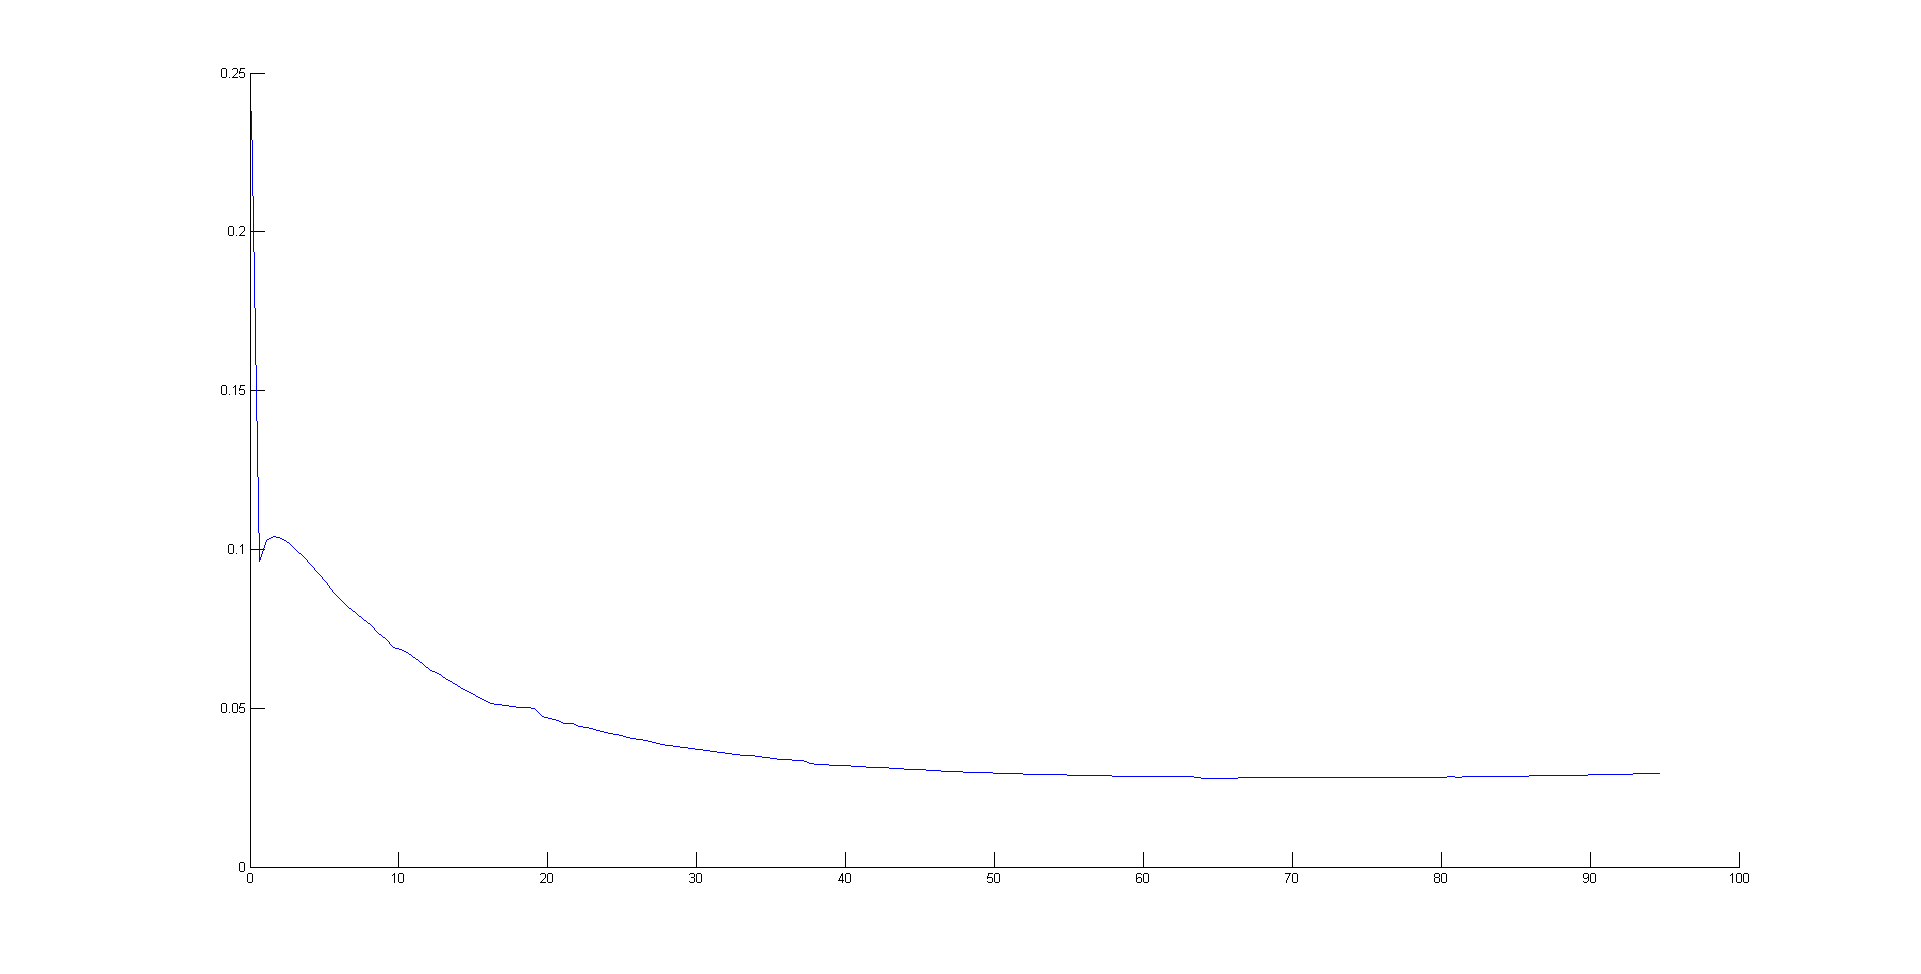
\includegraphics[width=130mm]{CW2-regulatorPID-ti35-opt1.png}
	\caption{Wykres przebiegu funkcji $Q(T_{d})$ regulatora P dla $T_{i}=0.35$.}
    \label{fig:regulatorPIDti35opt1}
\end{figure}
\begin{figure}[!h]
    \centering
	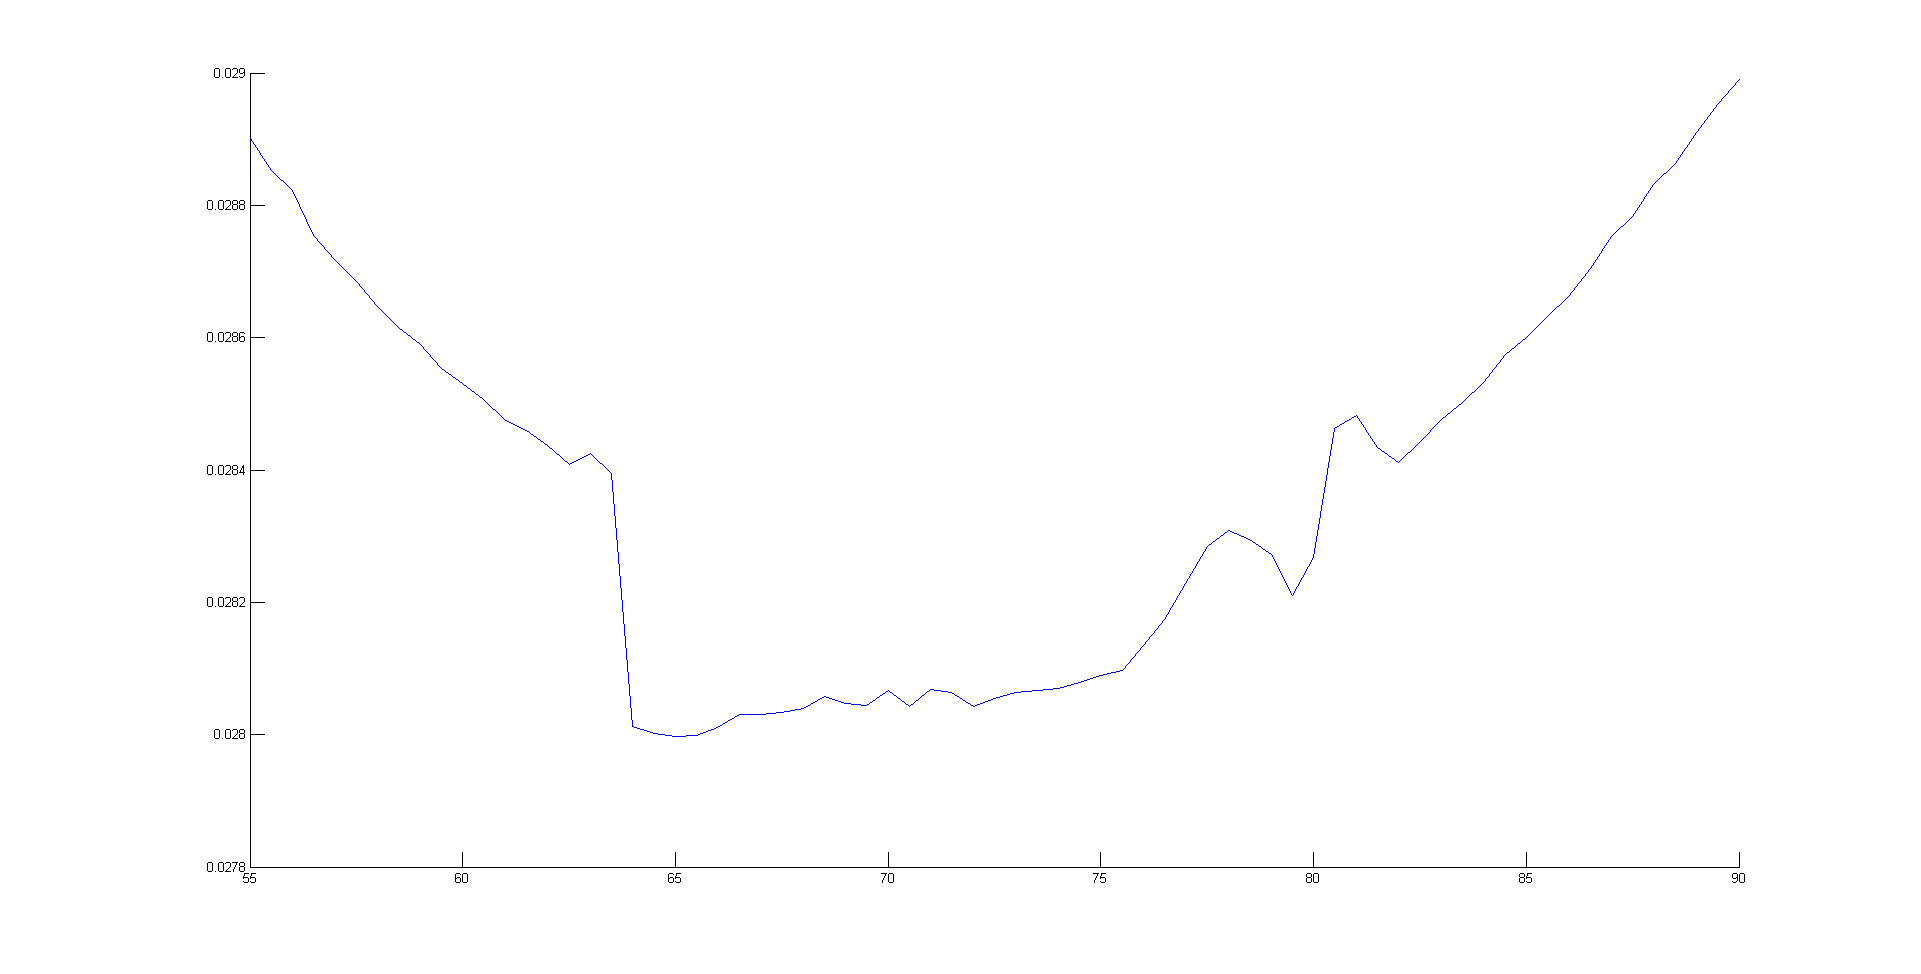
\includegraphics[width=130mm]{CW2-regulatorPID-ti35-opt2.png}
	\caption{Wykres przebiegu funkcji $Q(T_{d})$ regulatora P dla $T_{i}=0.35$ (powiększenie).}
    \label{fig:regulatorPIDti35opt2}
\end{figure}
\begin{figure}[!h]
    \centering
	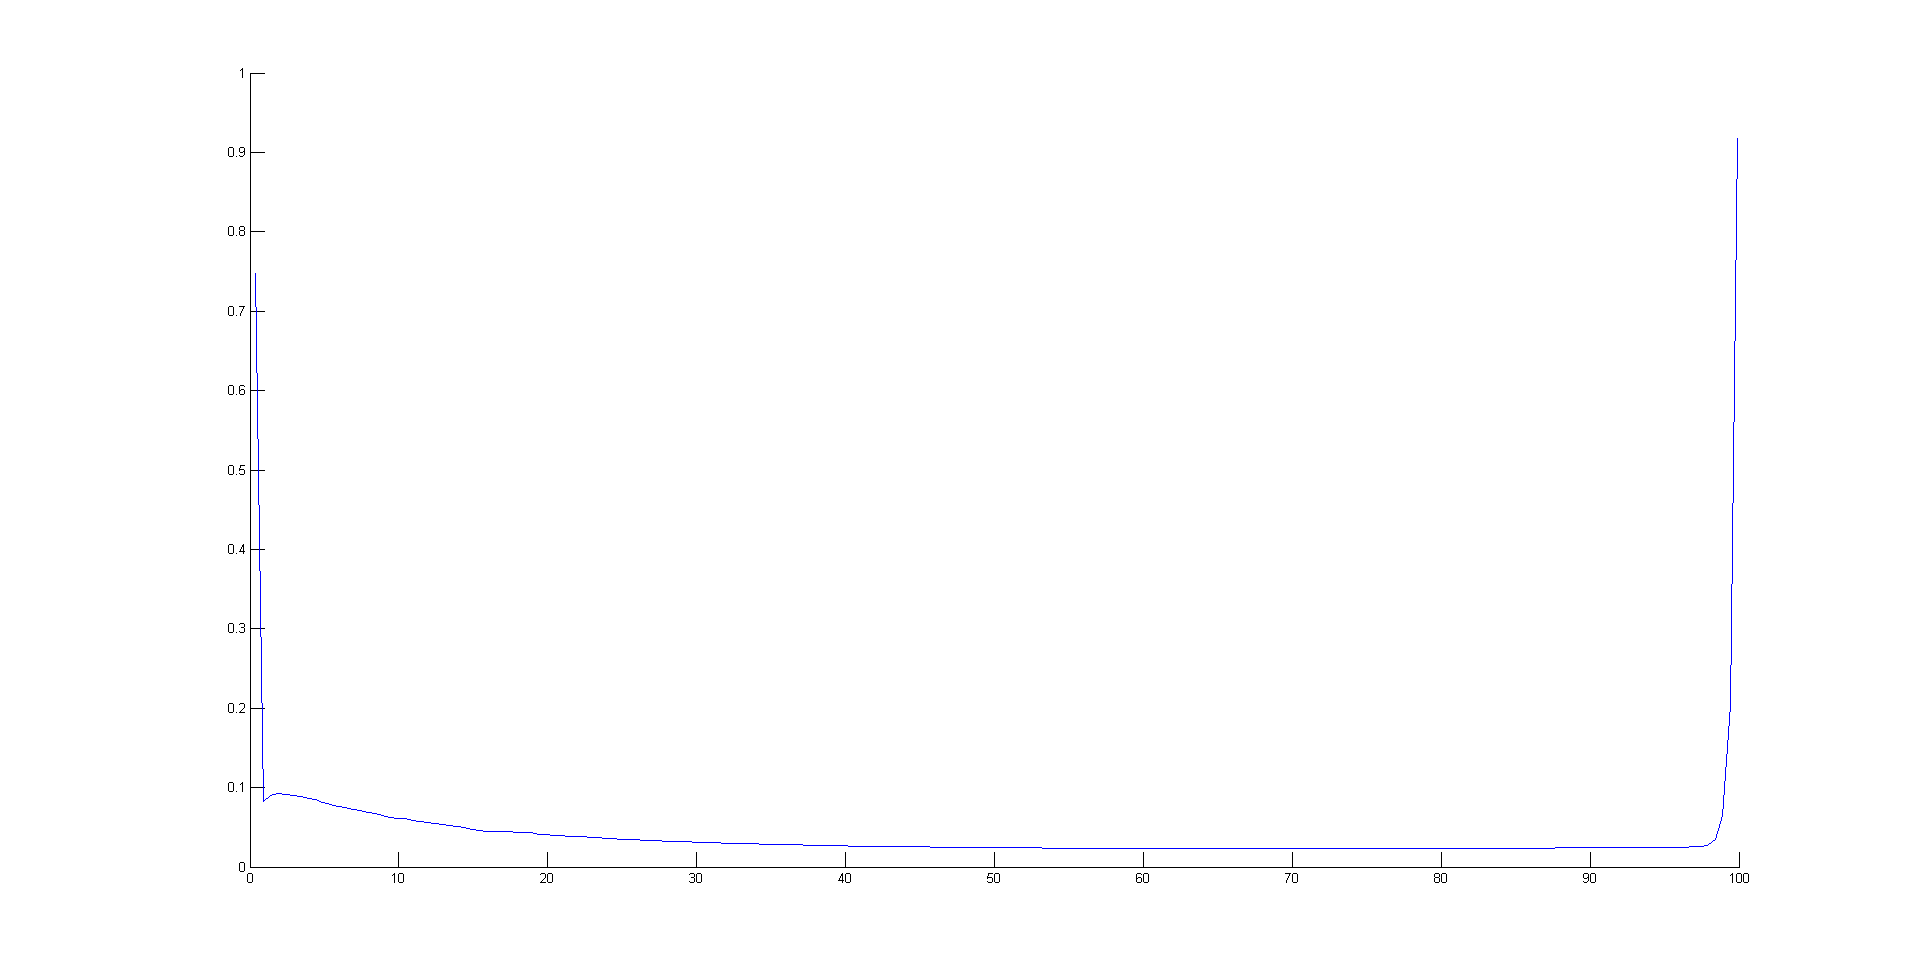
\includegraphics[width=130mm]{CW2-regulatorPID-ti100-opt1.png}
	\caption{Wykres przebiegu funkcji $Q(T_{d})$ regulatora P dla $T_{i}=1$.}
    \label{fig:regulatorPIDti100opt1}
\end{figure}
\begin{figure}[!h]
    \centering
	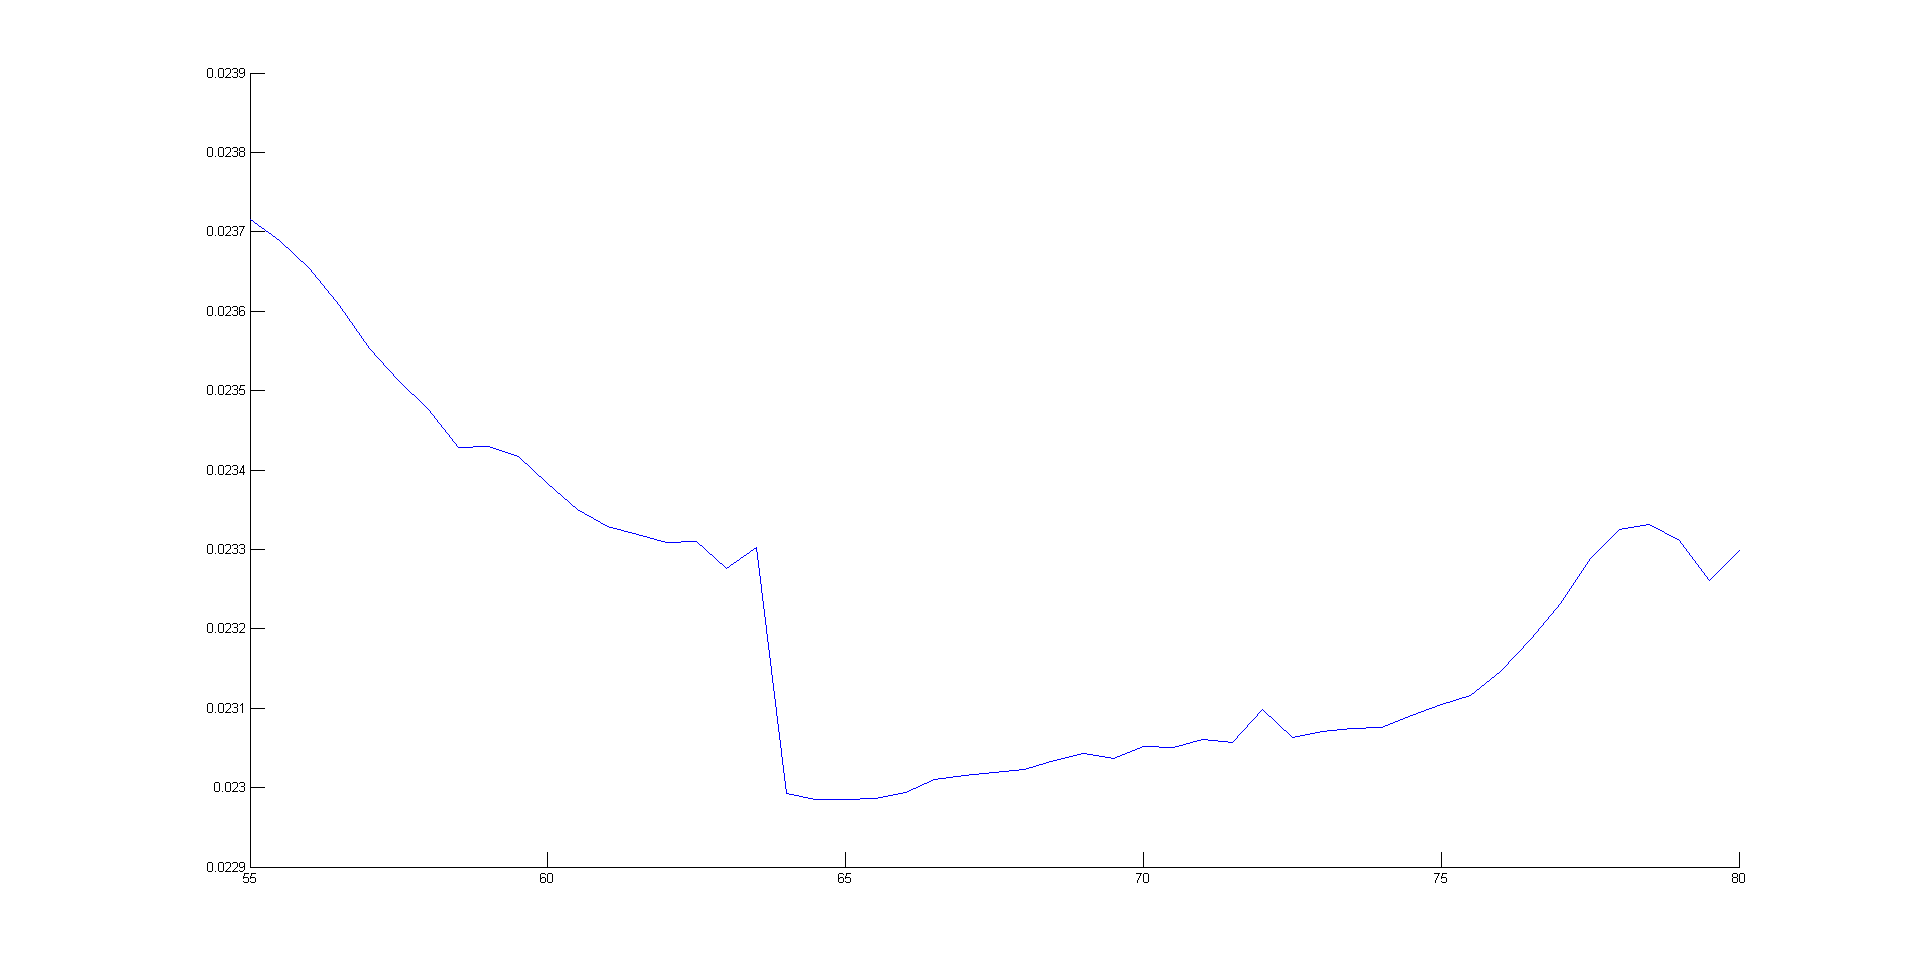
\includegraphics[width=130mm]{CW2-regulatorPID-ti100-opt2.png}
	\caption{Wykres przebiegu funkcji $Q(T_{d})$ regulatora P dla $T_{i}=1$ (powiększenie).}
    \label{fig:regulatorPIDti100opt2}
\end{figure}
\newpage Wartością optymalną parametru $T_{d}$ jest minimum funkcji $Q(T_{d})$, więc z wykresu \ref{fig:regulatorPIDti15opt1}, \ref{fig:regulatorPIDti15opt2}, \ref{fig:regulatorPIDti35opt1}, \ref{fig:regulatorPIDti35opt2}, \ref{fig:regulatorPIDti100opt1}, oraz \ref{fig:regulatorPIDti100opt2} możemy odczytać, że zarówno dla $T_{i}=0.15$ jak i dla $T_{i}=0.35$, oraz $T_{i}=1, T_{d} \approx 65$.

\subsection{Zastosowanie zasad Zieglera-Nicholsa.}\label{sec:zad3}
Doświadczalnie znalezienie współczynnika wzmocnienia dla którego układ traci stabilność.
Ustalenie Okresu oscylacji oraz wzmocnienia krytycznego.
Określić wartości parametrów regulatora PID.\\
\\
Wartości parametrów:\\
$T_{i}=9$\\
$T_{d}=3$\\
\\
Po wielu próbach otrzymaliśmy wynik, który  pokazuje, że dla wartości k=0.5 układ jest niestabilny. Co jest pokazane na wykresach.\\

\begin{figure}[!h]
    \centering
	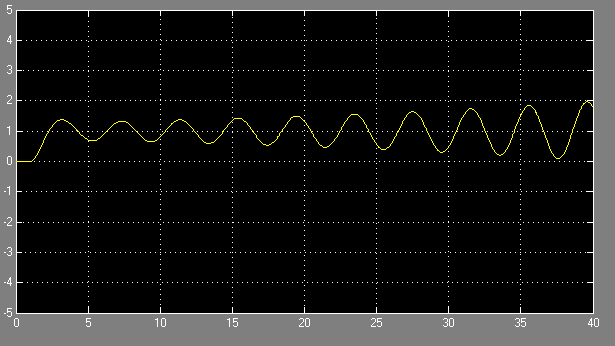
\includegraphics[width=130mm]{CW2-Z3-y.png}
	\caption{Charakterystyka y(t) dla układu niestablinego}
    \label{fig:z3-fy}
\end{figure}
\begin{figure}[!h]
    \centering
	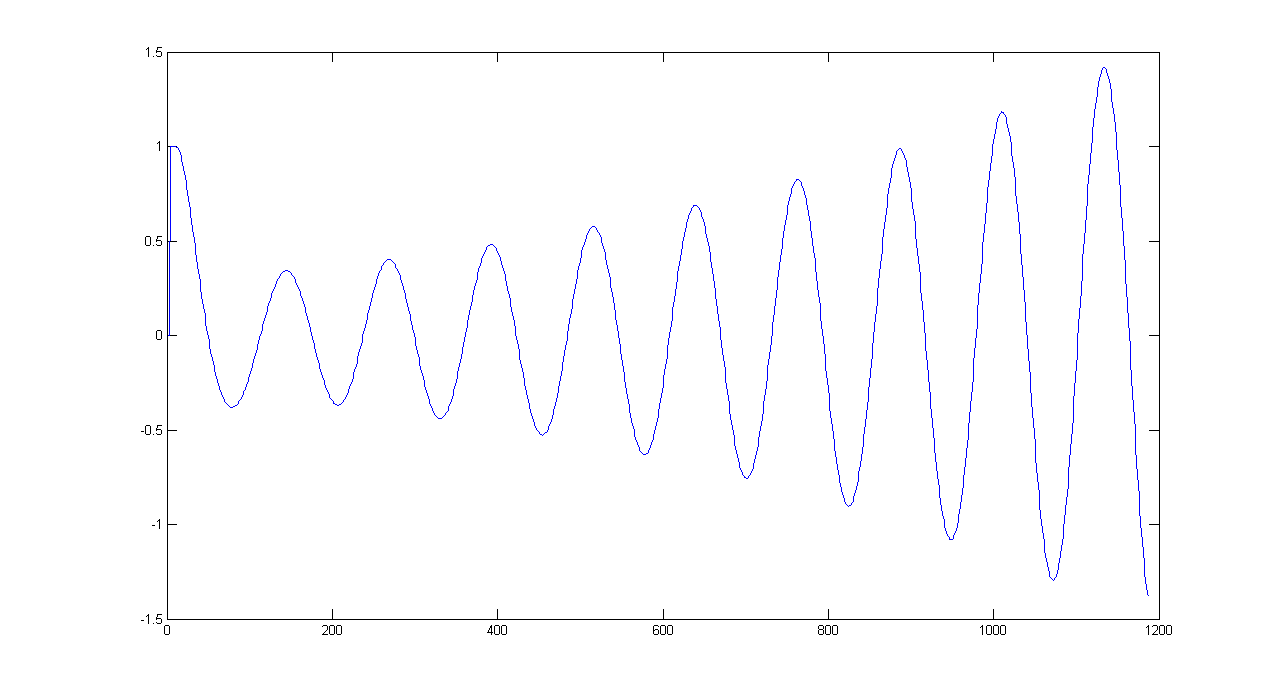
\includegraphics[width=130mm]{CW2-Z3-e.png}
	\caption{Charakterystyka e(t) dla układu niestablinego}
    \label{fig:z3-fe}
\end{figure}
\newpage
Aby wyznaczyć okres oscylacji oraz wzmocnienie krytyczne, korzystamy z metody  strojenia Zieglera-Nicholsa. W tej metodzie kryterium strojenia odbywa się poprzez ocenę układu, który znajduje się na granicy stabilności.
Metoda ta może być zastosowana tylko w wypadku gdy możliwe jest znalezienie wzmocnienia przy którym wykres Nyquista przecina punkt krytyczny lub linia pierwiastka przecina oś liczb urojonych. Najprościej to ustalić eksperymentalnie (muszą występować oscylacje o stałej amplitudzie)

\begin{figure}[!h]
\begin{tabular}{ | l | c | c | c | c | c | c | }
\hline
  Typ regulatora & \multicolumn{6}{|c|}{Optymalne wartości parametrów} \\   \hline
   & \multicolumn{3}{|c|}{Próba skokowa} & \multicolumn{3}{|c|}{Granica stabilności} \\   \hline
   & $K_{p}$ & $T_{i}$ & $T_{d}$ & $K_{p}$ & $T_{i}$ & $T_{d}$\\   \hline
   P & 1/a & - & - & $0.5K_{kr}$ & - & - \\   \hline
   PI & 0.9/a & $3 T_{d}$ & - & $0.45K_{kr}$ & $T_{osc}/1.2$ & - \\   \hline
   PID & 1.2/a & $2T_{d}$ & $0.5T_d$ & $0.6K_{kr}$ & $T_{osc}/2$ & $T_{osc}/8$ \\   \hline
\hline
\end{tabular}
	\caption{Tabela Zieglera-Nicholsa}
\end{figure}

Doświadczalnie wyznaczyliśmy, że układ znajduje się na granicy stabilności dla k=1.8 
\begin{figure}[htbp]
    \centering
	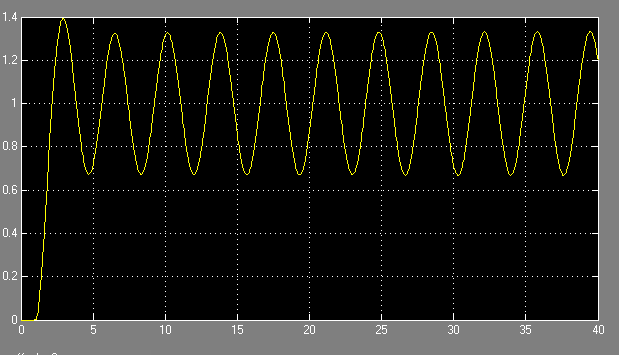
\includegraphics[width=130mm]{CW2-Z3-y2.png}
	\caption{Charakterystyka y(t) dla układu na granicy stabilności}
    \label{fig:z3-fy2}
\end{figure}
\begin{figure}[htbp]
    \centering
	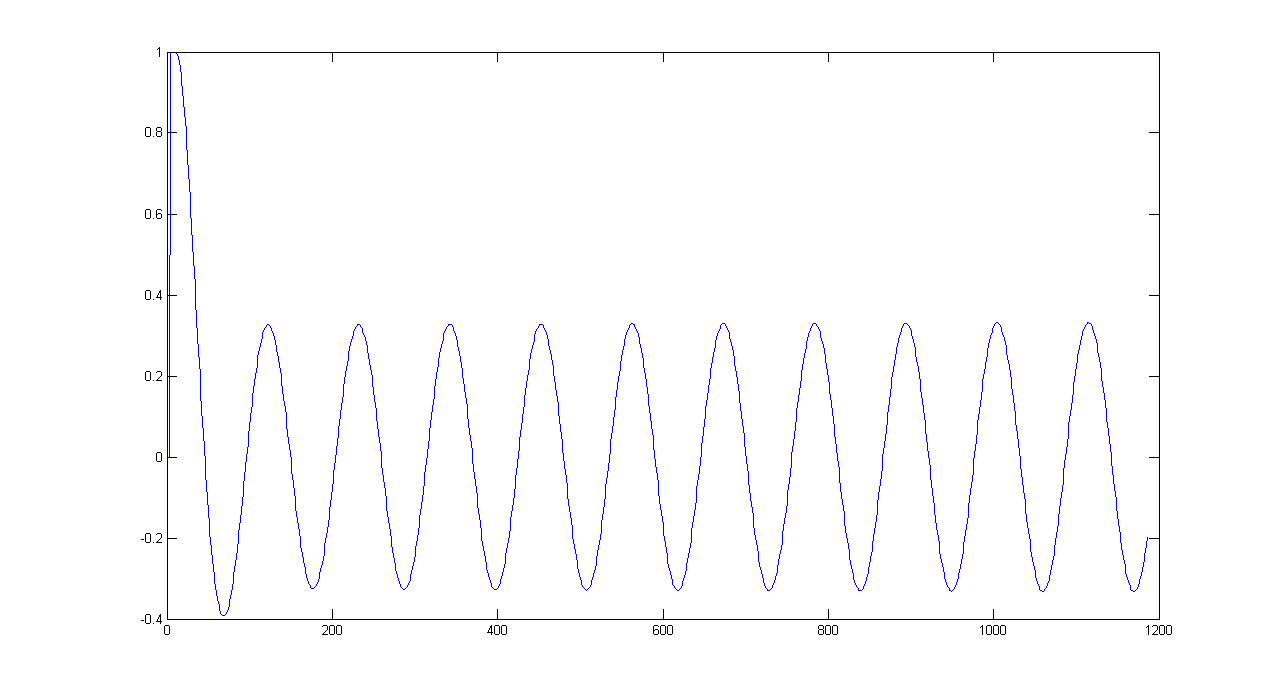
\includegraphics[width=130mm]{CW2-Z3-e2.png}
	\caption{Charakterystyka e(t) dla ukłądu na granicy stabilności}
    \label{fig:z3-fe2}
\end{figure}

Na podstawie wykresy można wyznaczyć $T_{osc}$
\begin{figure}[!h]
    \centering
	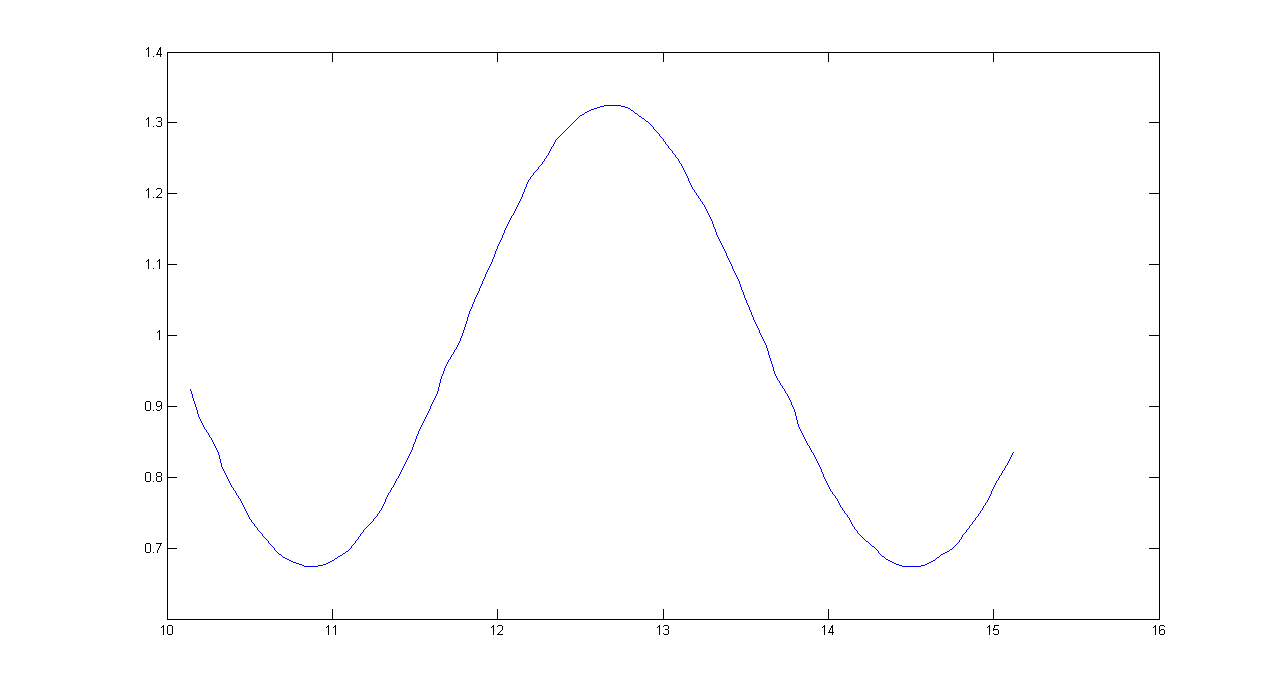
\includegraphics[width=130mm]{CW2-Z3-tosc.png}
	\caption{Charakterystyka y(t) do wyznaczenia Tosc}
    \label{fig:z3-fe2}
\end{figure}
\newline
Które wynosi:\\
Tosc=2.7
\newline
Otrzymany wynik to:\\
\begin{eqnarray}
\nonumber k=1.08\\
\nonumber Ti=1.35\\
\nonumber Td=0,4375\\
\end{eqnarray}
\newpage
Uzyskana charakterystyka to:\\
\begin{figure}[!h]
    \centering
	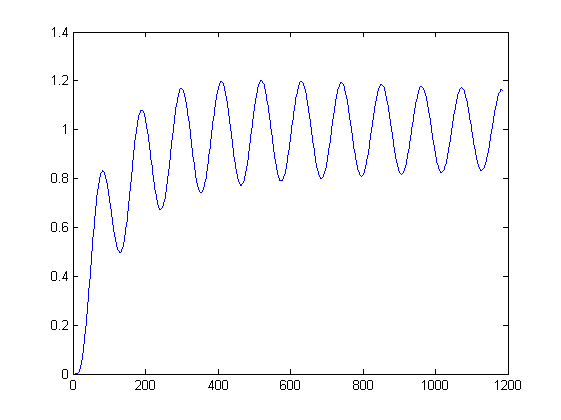
\includegraphics[width=130mm]{CW2-Z3-wyn.png}
	\caption{Charakterystyka y(t)}
    \label{fig:z3-wyn}
\end{figure}
\newpage
\section{Wnioski}
Po wykonaniu ćwiczenia zauważyliśmy pewne właściwości parametrów i jak ich zmiana wpływa na regulator. Sterowanie proporcionalne (k) ma wpływ na zmniejszenie czasu narastania oraz zmniejszanie uchybu, lecz nie daje dobrego efektu.
Zaś strowanie całkujące (Ti) ma wpływ na eliminowanie uchybu w stanie ustalonym, wadą zaś jest pogorszenie odpowiedzi w czasie narastania i przed czasem ustalonym. Sterowanie różniczkujące (Td) ma wpływ na zwiększenie stabilności układu, zmienijszając przeregulowanie i poprawiając odpowiedź między stanami. Dobór tych parametów jest niezwykle ważny dla układu regulacji, nieodpowiednie ich dobranie może powodować złe działanie lub nawet destabilizację układu.

\end{document}